
\documentclass[aspectratio=169]{beamer}
\usetheme{Boadilla}

\usepackage{qrcode}

\usepackage[utf8]{inputenc}       % Codificação de entrada
\usepackage[T1]{fontenc}          % Codificação de saída
\usepackage[portuguese]{babel}   % Idioma
\usepackage{XCharter}             % Fonte principal
\AtBeginDocument{\fontsize{12}{12}\selectfont}

%\usepackage{geometry}
%\geometry{papersize={210mm,150mm}}
\usepackage{tikz}
\usepackage{pgf-pie} % necessário para gráficos de pizza

\usepackage{color}
\usepackage{graphicx}
\usepackage{amsmath, amssymb, amsfonts}
\usepackage{bm}
\usepackage{booktabs}
\usepackage{multirow}
\usepackage{caption}
\usepackage{subfigure}
\usepackage{wrapfig}
\usepackage{multicol}
\usepackage{sidecap}
\usepackage{tikz}
\usepackage{listings}
\usepackage{siunitx}
\usepackage{pdfpages}
\usepackage{float}
\usepackage{hyperref}
\usepackage{academicons}
\usepackage{setspace}

\newcommand{\eng}[1]{\textsl{#1}}
\newcommand{\cod}[1]{\texttt{#1}}

\usepackage{tikz}
\usetikzlibrary{shapes.geometric, arrows, positioning}

% Definição de estilos para o fluxograma
\tikzstyle{startstop} = [ellipse, rounded corners, minimum width=2cm, minimum height=0.8cm, text centered, draw=black, fill=gray!20]
\tikzstyle{process} = [rectangle, minimum width=3.5cm, minimum height=1cm, text width=4.5cm, text centered, draw=black, fill=white]
\tikzstyle{decision} = [diamond, aspect=2, minimum width=3cm, minimum height=1cm, text centered, draw=black, fill=white]
\tikzstyle{arrow} = [thick,->,>=stealth]

% Definição de cores profissionais
\definecolor{mipsblue}{RGB}{50, 90, 120}
\definecolor{mipsred}{RGB}{150, 30, 30}

\title[Arquitetura de Computadores]{\huge  Hardware Description Languages} %note that the optional arg in '[]' are displayed in the left column throughout the complete presentation
% adapt accordingly
% e.g., M.Sc. Intermediate Thesis Report
% or     B.Sc. Intermediate Thesis Report


\author[Prof. Dr. Oscar Eduardo Anacona Mosquera]{Prof. Dr. Oscar Eduardo Anacona Mosquera \newline\newline 
	\scriptsize{oscar.mosquera@ufmt.br}
}%note that the optional arg in '[]' are displayed in the left column throughout the complete presentation



\AtBeginSection[]
{
	\begin{frame}{Sumário}
		\tableofcontents[currentsection]
	\end{frame}
}


\begin{document}

	\begin{frame}[plain]
		\titlepage
	\end{frame}
	
	\begin{frame}{Sumário}
		\tableofcontents
	\end{frame}
	
%=======================================================================================
%\section{Introdução}
%=======================================================================================


\section{Introdução}


\begin{frame}{VHDL}
	\justifying
	
	\begin{block}{}
		\justifying
		A VHDL permite que os engenheiros descrevam o comportamento e a estrutura de circuitos digitais complexos. Essa descrição pode incluir informações sobre sinais, portas, componentes, processos, temporização e outros aspectos do projeto.
	\end{block}
	
	\begin{itemize}
		\item \textbf{V}HSIC (Very High Speed Integrated Circuit)
		\item \textbf{H}ardware
		\item \textbf{D}escription
		\item \textbf{L}anguage
	\end{itemize}
	
	\begin{alertblock}{}
		``\textbf{Tell me how your circuit should behave and I will give you
			hardware that does the job.}”
	\end{alertblock}	
	
	
\end{frame}


\begin{frame}{Histórico e Padronização}
	\justifying
	VHDL significa \textit{VHSIC (Very High Speed Integrated Circuits) Hardware Description Language}, resultado de uma iniciativa do Departamento de Defesa dos EUA na década de 1980.
	
	\begin{itemize}
		\item \textbf{Evolução:} Surgiu como VHDL 87, seguido pelas versões 93, 2002 e 2008.
		\item \textbf{Padrão IEEE:} Foi a primeira HDL padronizada (IEEE 1076 e 1164).
		\item \textbf{Portabilidade:} A linguagem é independente de tecnologia ou fabricante, tornando os códigos reutilizáveis e portáveis.
	\end{itemize}
\end{frame}









\begin{frame}{Principais características}
	\justifying
	
	\begin{itemize}
		\justifying
		\item \textbf{Descrição de Hardware:} VHDL permite a descrição abstrata de sistemas digitais, abrangendo desde níveis mais altos de comportamento até detalhes de baixo nível.
		\item \textbf{Simulação e Verificação:} A linguagem é amplamente utilizada em simulação para verificar o comportamento e o desempenho dos projetos antes da implementação física.
		\item \textbf{Síntese Lógica:} VHDL é frequentemente utilizado em conjunto com ferramentas de síntese para transformar a descrição de alto nível em uma implementação específica em hardware.
		\item \textbf{Projeto de Circuitos Complexos:} É particularmente útil para projetar sistemas digitais complexos, como processadores, sistemas embarcados, e outros dispositivos eletrônicos.
		
	\end{itemize}
	
	
\end{frame}




\begin{frame}{Principais características}
	\justifying
	
	\begin{itemize}
		\justifying
		
		\item \textbf{Reutilização de Design:} A VHDL suporta a reutilização de design, permitindo que módulos e componentes sejam definidos e posteriormente utilizados em diferentes projetos
		\item \textbf{Padrão IEEE:} VHDL é um padrão IEEE (\textbf{Institute of Electrical and Electronics Engineers}), o que contribui para sua ampla aceitação e uso na indústria.
		\item \textbf{Síntese para FPGAs e ASICs:} Pode ser utilizado para a síntese de projetos em FPGAs ou ASICs, convertendo a descrição em hardware físico.
	\end{itemize}
	
	
\end{frame}




\begin{frame}{Terminologia}
	\justifying
	
	\begin{itemize}
		\justifying
		\item \textbf{HDL:} uma limguagem de descrição de hardware é uma linguagem de programação de software usada para a modelagem de um circuito hardware.
		
		\item \textbf{Modelo comportamental:} um componente é descrito pela resposta das entradas e saídas.
		
		\item \textbf{Modelo estrutural:} um componente é descrito pela interconexão de componentes/primitivas de níveis mais baixos (\textbf{abordagem top-down design}).
		
		
	\end{itemize}
	
	
\end{frame}



\begin{frame}{Modelo comportamental (Behavioral Modeling)}
	\justifying
	
	\begin{itemize}
		\justifying
		\item Somente a funcionalidade do circuito, não a estrutura.
		
		\item A descrição do hardware não está vinculada a uma implementação específica de hardware.
		
		
		
	\end{itemize}
	
	
	\begin{figure}[h]
		\centering
		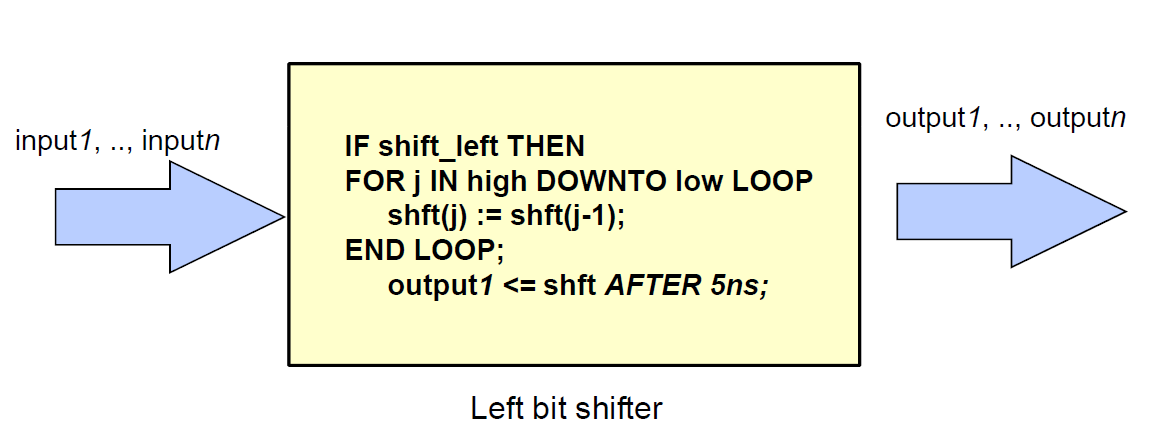
\includegraphics[width=0.67\textwidth]{Figs/fig03.png}
	\end{figure}
	
	
\end{frame}

\begin{frame}{Modelo estrutural (Structural Modeling)}
	\justifying
	
	\begin{itemize}
		\justifying
		\item Funcionalidade e estrutura do circuito.
	\end{itemize}
	
	
	\begin{figure}[h]
		\centering
		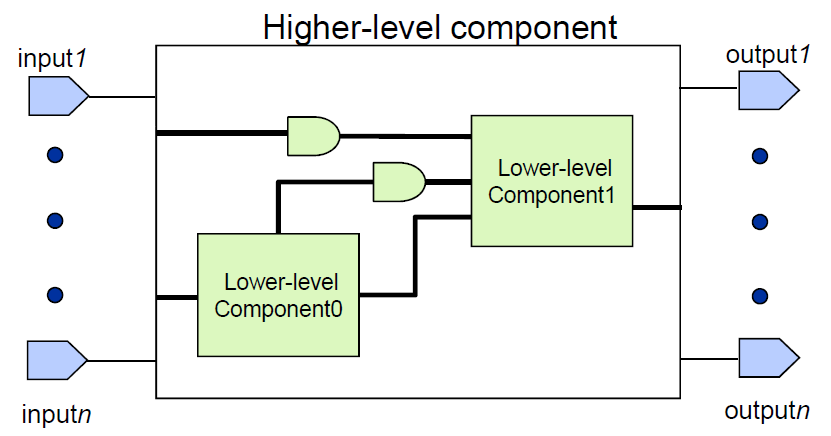
\includegraphics[width=0.67\textwidth]{Figs/fig04.png}
	\end{figure}
	
	
\end{frame}


\begin{frame}{Terminologia}
	\justifying
	
	\begin{itemize}
		\justifying
		\item \textbf{Register Transfer Level (RTL):} um tipo de modelo comportamental, com o propósito de síntese. O hardware é implícito e é sintetizável.
		
		\item \textbf{Síntese:} traduzindo HDL para um circuito e, em seguida, otimizando o circuito representado.
		
		\item \textbf{Processo:} unidade básica de execução em VHDL (são convertidos para seu equivalente em hardware).
		
		
	\end{itemize}
	
	
\end{frame}


\begin{frame}{RTL Synthesis}
	\justifying
	
	
	\begin{figure}[h]
		\centering
		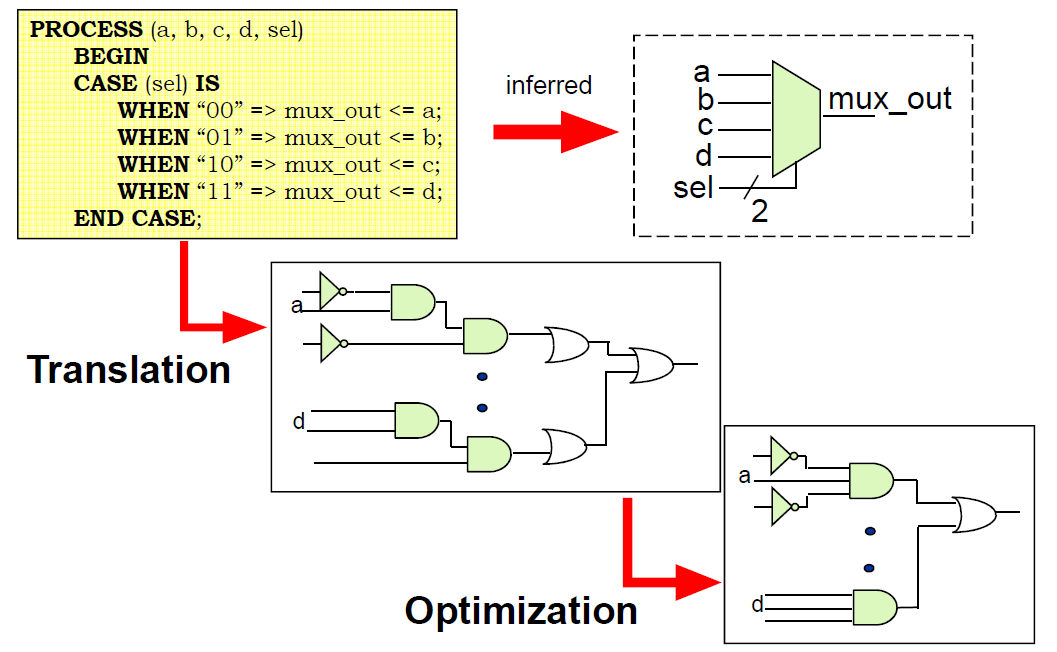
\includegraphics[width=0.75\textwidth]{Figs/fig05.png}
	\end{figure}
	
	
\end{frame}



\begin{frame}{Translation of VHDL Code into a Circuit}
	\justifying
	
	
	\begin{figure}[h]
		\centering
		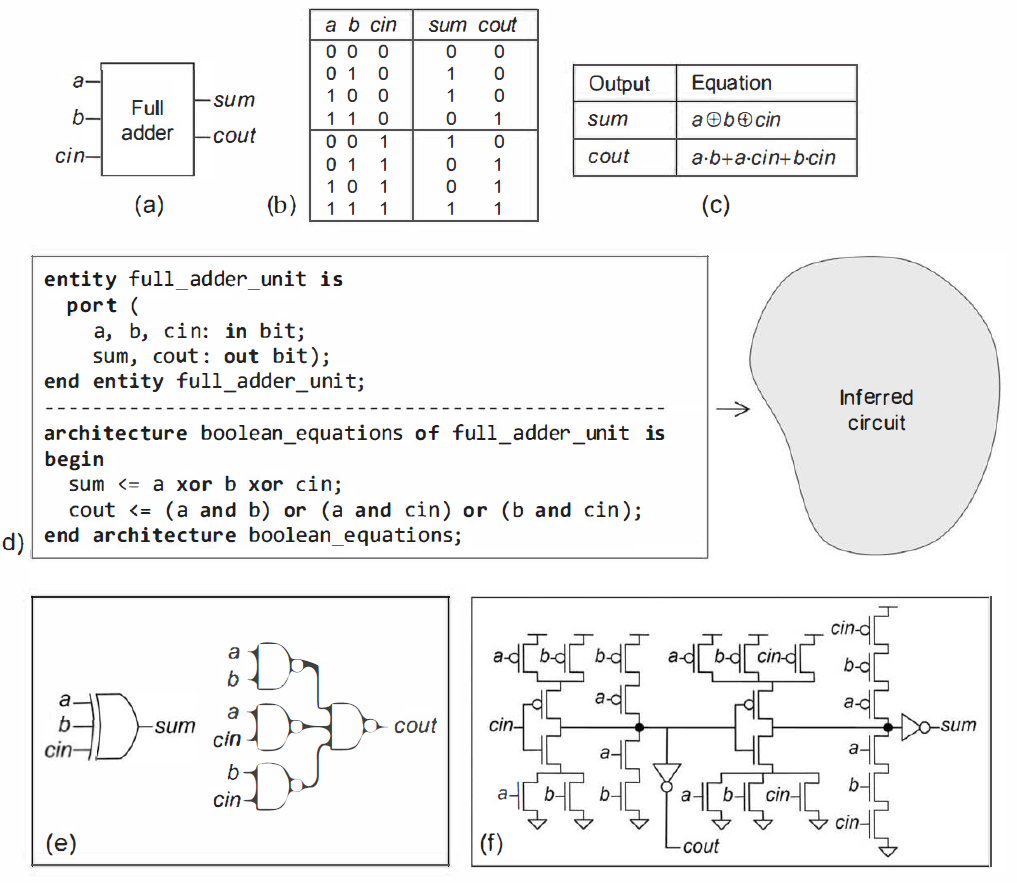
\includegraphics[width=0.5\textwidth]{Figs/fig93.png}
	\end{figure}
	
	
\end{frame}



\section{Estrutura do Código}


\begin{frame}{Unidades de Design VHDL}
	\justifying
	
	\begin{itemize}
		\justifying
		\item \textbf{Entidades (Entities):} Entidades definem a interface do componente, especificando seus sinais de entrada e saída. Elas são como um contrato que descreve o comportamento externo do componente. As entidades não contêm lógica interna.
		
		\item \textbf{Arquiteturas (Architectures):} Arquiteturas definem a lógica interna de uma entidade. Elas descrevem como os sinais de entrada são manipulados para produzir os sinais de saída. Uma entidade pode ter várias arquiteturas, cada uma representando uma implementação diferente.
		
%		\item \textbf{Pacotes (Packages):} Pacotes são usados para agrupar constantes, tipos de dados, subprogramas e outras declarações que podem ser compartilhadas entre várias entidades e arquiteturas. Eles são úteis para promover a reutilização e a organização do código.
		
		
		
	\end{itemize}
	
	
\end{frame}



\begin{frame}{Declaração da Entidade}
	\justifying
	
	
	\begin{figure}[h]
		\centering
		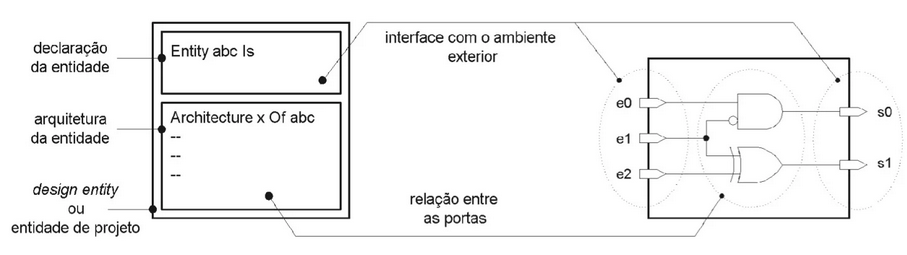
\includegraphics[width=1\textwidth]{Figs/fig09.png}
	\end{figure}
	
	
\end{frame}



\begin{frame}{Declaração da Entidade}
	\justifying
	
	
	\begin{figure}[h]
		\centering
		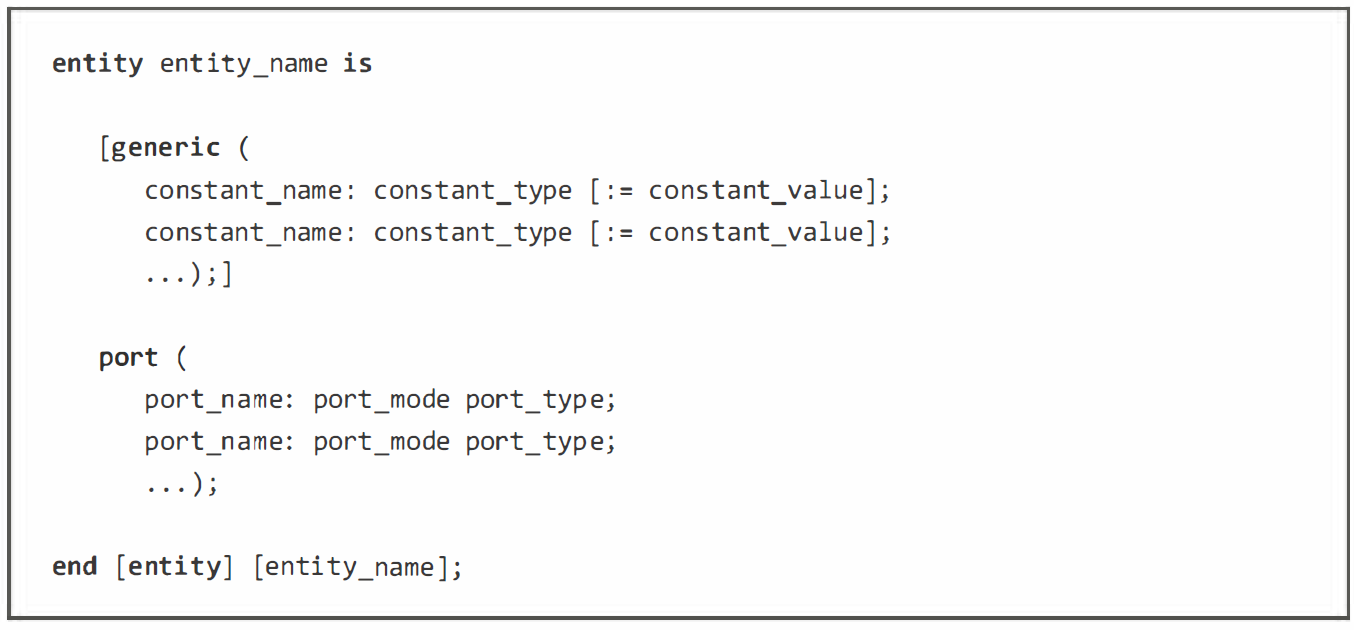
\includegraphics[width=0.97\textwidth]{Figs/fig11.png}
	\end{figure}
	
	
\end{frame}


\begin{frame}{Declaração da Entidade}
	\justifying
	
	Há quatro modos possíveis de uma porta, são eles:
	
	\begin{itemize}
		\item \textbf{IN:} porta de entrada.
		\item \textbf{OUT:} porta de saída, não pode ser referenciado internamente pela arquitetura.
		\item \textbf{BUFFER:} a porta opera unicamente no modo saída, pode ser referenciado internamente pela arquitetura.
		\item \textbf{INOUT:} caracteriza uma porta bidirecional onde uma informação pode ser apresentada ou amostrada.
	\end{itemize}
	
	
	
\end{frame}



\begin{frame}{Corpo da arquitetura}
	\justifying
	
	
	
	\begin{figure}[h]
		\centering
		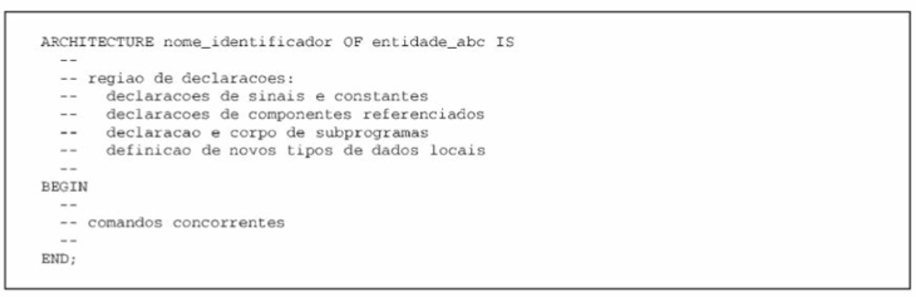
\includegraphics[width=0.97\textwidth]{Figs/fig14.png}
	\end{figure}
	
	
	
\end{frame}


\begin{frame}{Corpo da arquitetura}
	\justifying
	
	
	\begin{figure}[h]
		\centering
		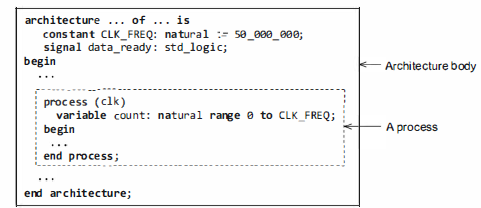
\includegraphics[width=0.97\textwidth]{Figs/fig29.png}
	\end{figure}
	
	
	
\end{frame}
%------------
\begin{frame}{Corpo da arquitetura}
	\justifying
	
	
	\begin{figure}[h]
		\centering
		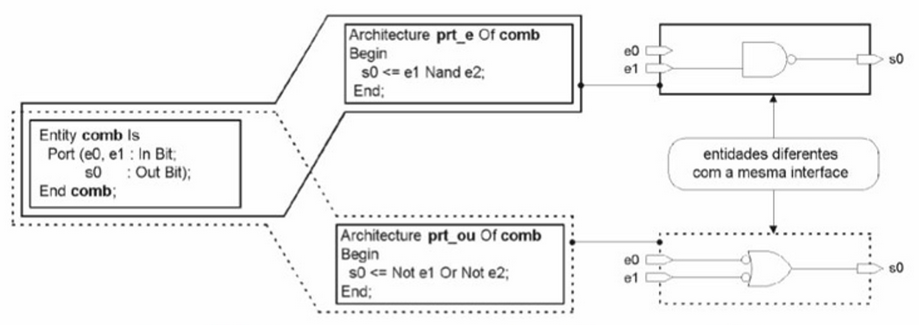
\includegraphics[width=0.97\textwidth]{Figs/fig15.png}
	\end{figure}
	
	
	
\end{frame}













% --- FRAME 1 (Parte 1/2) ---



%\begin{frame}{Visão Geral do VHDL}
%	\justifying
%	VHDL é uma linguagem de descrição de hardware utilizada para descrever o comportamento ou a estrutura de circuitos eletrônicos. A partir do código, um compilador infere um circuito físico equivalente. 
%	
%	Suas principais aplicações incluem:
%	\begin{itemize}
%		\item Síntese de circuitos digitais em dispositivos lógicos programáveis (CPLD/FPGA).
%		\item Geração de layout e máscaras para fabricação de circuitos integrados de aplicação específica (ASIC).
%	\end{itemize}
%	O VHDL permite tanto a \textbf{síntese} (tradução para hardware) quanto a \textbf{simulação} (procedimento de teste para garantir a funcionalidade).
%\end{frame}










% --- FRAME 10 ---





% --- FRAME 11 ---
\begin{frame}{Fluxo de Projeto (Design Flow)}
	\justifying
	O fluxo simplificado consiste em: escrever o código (.vhd), compilar para síntese, realizar o \textit{fitting} (alocação física no chip) e simular para verificar o comportamento temporal.
	
	\begin{figure}[h]
		\centering
		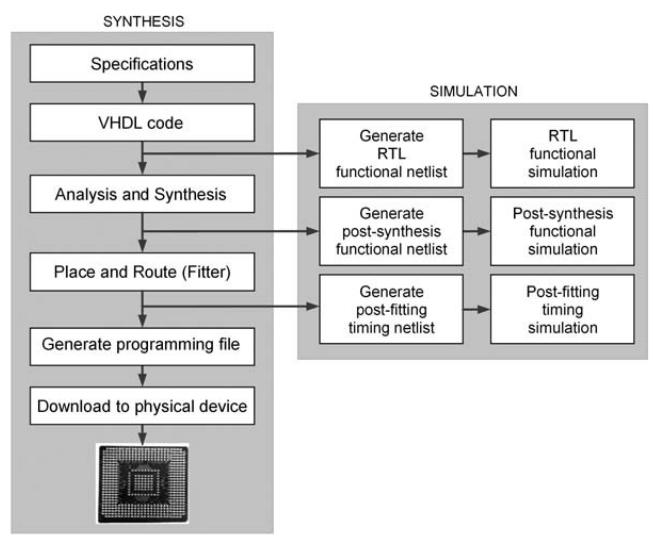
\includegraphics[width=0.5\textwidth]{Figs/new_fig03.png}
		%\caption{Fluxo de projeto simplificado em VHDL.}
	\end{figure}
\end{frame}

% --- FRAME 12 ---
\begin{frame}{Ferramentas EDA}
	\justifying
	Existem diversas ferramentas de Automação de Design Eletrônico (EDA) para síntese e simulação:
	
	\begin{itemize}
		\item \textbf{Fabricantes de FPGA:} Altera (Quartus II) e Xilinx (Vivado/ISE).
		\item \textbf{Softwares de Terceiros:} Mentor Graphics (ModelSim), Synopsys (VCS/Synplify) e Cadence (NC-Sim).
	\end{itemize}
	As ferramentas de fabricantes geralmente oferecem versões gratuitas (\textit{Web Edition}) para fins educacionais.
\end{frame}



\begin{frame}{Experimento 1}
	\justifying
	Portas AND
\end{frame}











\section{Tipos de dados}



\begin{frame}{Tipos de dados}
	\justifying
	
	
	
	\begin{figure}[h]
		\centering
		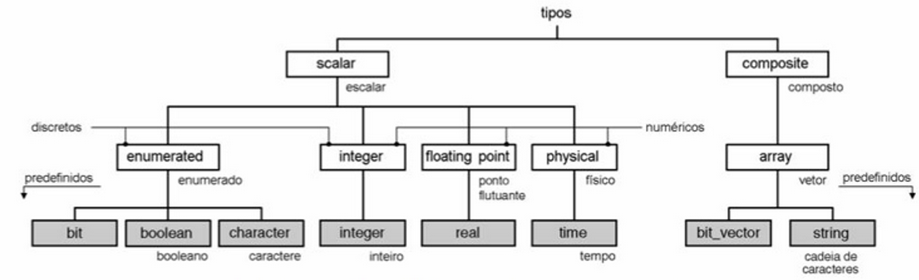
\includegraphics[width=0.97\textwidth]{Figs/fig21.png}
	\end{figure}
	
	
	
	%	\begin{figure}[h]
		%		\centering
		%		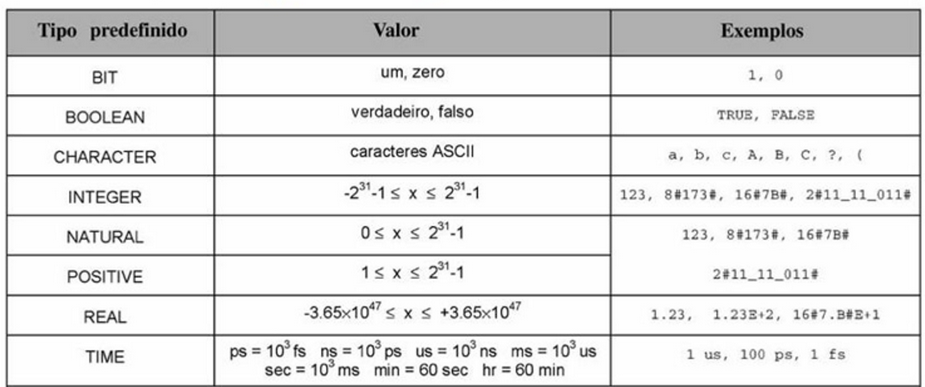
\includegraphics[width=0.77\textwidth]{Figs/fig22.png}
		%	\end{figure}	
	
\end{frame}


\begin{frame}{Tipos de dados}
	\justifying
	
	
	
	%	\begin{figure}[h]
		%		\centering
		%		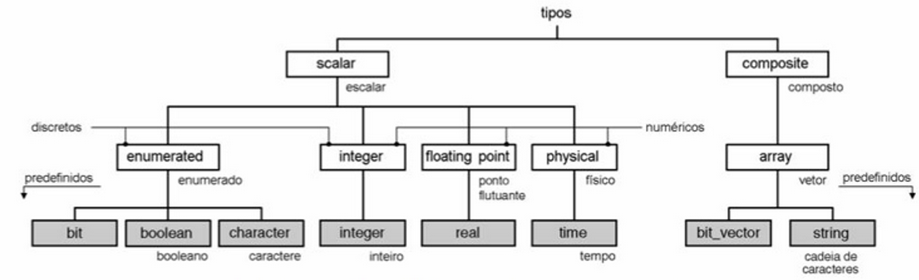
\includegraphics[width=0.97\textwidth]{Figs/fig21.png}
		%	\end{figure}
	
	
	
	\begin{figure}[h]
		\centering
		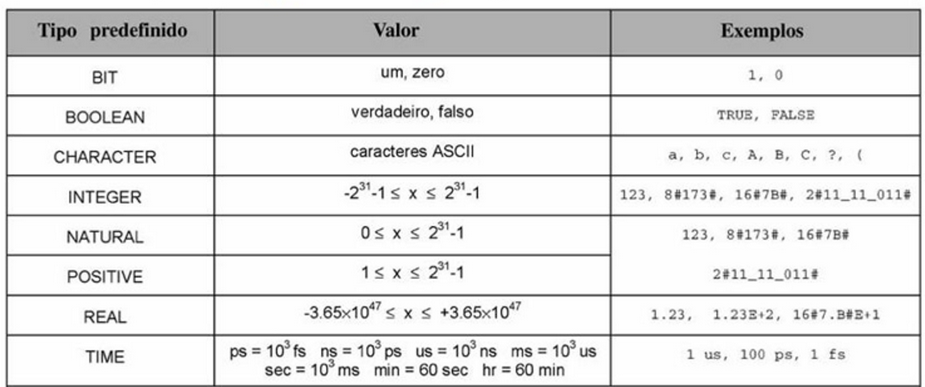
\includegraphics[width=0.9\textwidth]{Figs/fig22.png}
	\end{figure}	
	
\end{frame}





\begin{frame}{Experimento 2}
	\justifying
	Sistemas numéricos
\end{frame}
















%\section{Estrutura do Código}
%
%
%\begin{frame}{Unidades de Design VHDL}
%	\justifying
%	
%	\begin{itemize}
%		\justifying
%		\item \textbf{Entidades (Entities):} Entidades definem a interface do componente, especificando seus sinais de entrada e saída. Elas são como um contrato que descreve o comportamento externo do componente. As entidades não contêm lógica interna.
%		
%		\item \textbf{Arquiteturas (Architectures):} Arquiteturas definem a lógica interna de uma entidade. Elas descrevem como os sinais de entrada são manipulados para produzir os sinais de saída. Uma entidade pode ter várias arquiteturas, cada uma representando uma implementação diferente.
%		
%		\item \textbf{Pacotes (Packages):} Pacotes são usados para agrupar constantes, tipos de dados, subprogramas e outras declarações que podem ser compartilhadas entre várias entidades e arquiteturas. Eles são úteis para promover a reutilização e a organização do código.
%		
%		
%		
%	\end{itemize}
%	
%	
%\end{frame}



%\begin{frame}{Unidades de Design VHDL}
%	\justifying
%	
%	\begin{itemize}
%		\justifying
%		
%		
%		\item \textbf{Configurações (Configurations):} Configurações são usadas para associar uma entidade a uma arquitetura específica ou a outras entidades. Elas permitem configurar a hierarquia do projeto e selecionar as implementações desejadas para cada componente.
%		
%		\item \textbf{Bibliotecas (Libraries):} Bibliotecas são coleções de unidades de design relacionadas, como entidades, arquiteturas e pacotes. Elas ajudam a organizar e gerenciar o código, permitindo a reutilização de unidades em diferentes projetos.
%		
%		
%	\end{itemize}
%	
%	
%\end{frame}



%\begin{frame}{Unidades de Design VHDL}
%	\justifying
%	
%	
%	\begin{figure}[h]
%		\centering
%		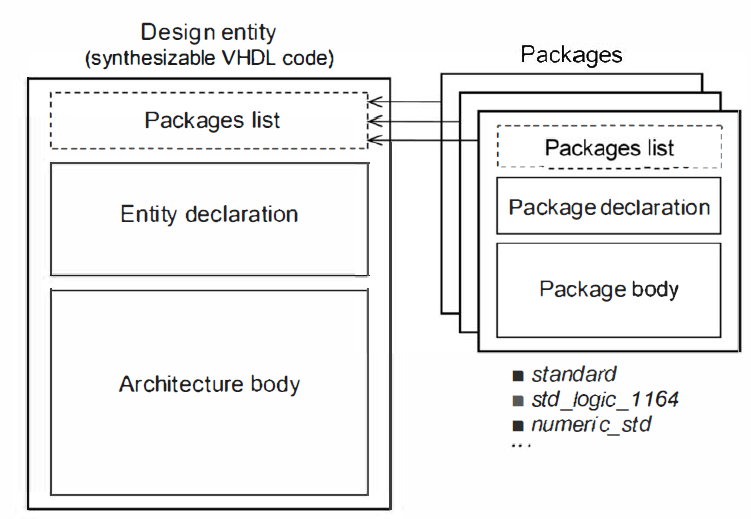
\includegraphics[width=0.7\textwidth]{Figs/fig10.png}
%	\end{figure}
%	
%	
%\end{frame}

%\begin{frame}{Declaração da Entidade}
%	\justifying
%	
%	
%	\begin{figure}[h]
%		\centering
%		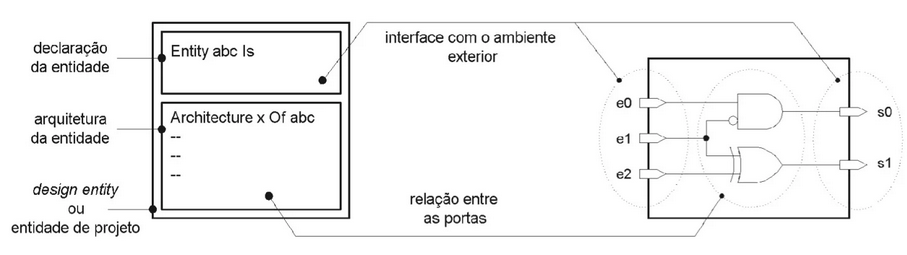
\includegraphics[width=1\textwidth]{Figs/fig09.png}
%	\end{figure}
%	
%	
%\end{frame}





% --- FRAME 2 ---
%\begin{frame}{Bibliotecas e Pacotes: Biblioteca \texttt{std}}
%	\justifying
%	As bibliotecas padrão são \texttt{std} e \texttt{ieee}. Na biblioteca \texttt{std}, destacam-se:
%	\begin{itemize}
%		\item \textbf{Package standard:} Parte integrante do VHDL desde 1987. Define tipos de dados básicos como \texttt{BIT, INTEGER, BOOLEAN, CHARACTER} e seus respectivos operadores lógicos e aritméticos.
%		\item \textbf{Package textio:} Provê recursos para manipulação de textos e arquivos.
%	\end{itemize}
%	Ambos os pacotes foram expandidos na revisão VHDL 2008 para oferecer maior suporte a novas funcionalidades.
%\end{frame}
%
%% --- FRAME 3 ---
%\begin{frame}{Bibliotecas e Pacotes: Biblioteca \texttt{ieee}}
%	\justifying
%	A biblioteca \texttt{ieee} contém os pacotes mais utilizados no design moderno:
%	\begin{itemize}
%		\item \textbf{std\_logic\_1164:} Define os tipos \texttt{STD\_LOGIC} (9 valores), permitindo o uso de alta impedância ('Z') e valores irrelevantes (\textit{don't care} '-').
%		\item \textbf{numeric\_std:} Introduz os tipos \texttt{SIGNED} e \texttt{UNSIGNED} baseados em \texttt{STD\_LOGIC}.
%		\item \textbf{Novidades VHDL 2008:} Introdução dos pacotes \texttt{fixed\_pkg} (ponto fixo) e \texttt{float\_pkg} (ponto flutuante), além de melhorias para operações sem sinal (\texttt{numeric\_std\_unsigned}).
%	\end{itemize}
%\end{frame}

% --- FRAME 4 ---
%\begin{frame}{Pacotes Não Padronizados}
%	\justifying
%	Alguns pacotes, embora populares, não fazem parte do padrão estrito da IEEE, mas são amplamente suportados por ferramentas de síntese:
%	\begin{itemize}
%		\item \textbf{std\_logic\_arith:} Equivalente parcial ao \texttt{numeric\_std}.
%		\item \textbf{std\_logic\_unsigned} e \textbf{std\_logic\_signed:} Permitem operações aritméticas diretamente sobre sinais do tipo \texttt{STD\_LOGIC\_VECTOR}, tratando-os como números sem sinal ou com sinal, respectivamente.
%	\end{itemize}
%	Recomenda-se priorizar o uso de pacotes padrão (\texttt{numeric\_std}) para garantir maior portabilidade do código.
%\end{frame}




\section{Librarias em VHDL}



\begin{frame}{Unidades de Design VHDL}
	\justifying
	
	\begin{itemize}
		\justifying
	%	\item \textbf{Entidades (Entities):} Entidades definem a interface do componente, especificando seus sinais de entrada e saída. Elas são como um contrato que descreve o comportamento externo do componente. As entidades não contêm lógica interna.
		
		%\item \textbf{Arquiteturas (Architectures):} Arquiteturas definem a lógica interna de uma entidade. Elas descrevem como os sinais de entrada são manipulados para produzir os sinais de saída. Uma entidade pode ter várias arquiteturas, cada uma representando uma implementação diferente.
		
		\item \textbf{Pacotes (Packages):} Pacotes são usados para agrupar constantes, tipos de dados, subprogramas e outras declarações que podem ser compartilhadas entre várias entidades e arquiteturas. Eles são úteis para promover a reutilização e a organização do código.
		
		
		
	\end{itemize}
	
	
\end{frame}

\begin{frame}{VHDL- pacotes std e IEEE}
	\justifying
	
	
	
	\begin{figure}[h]
		\centering
		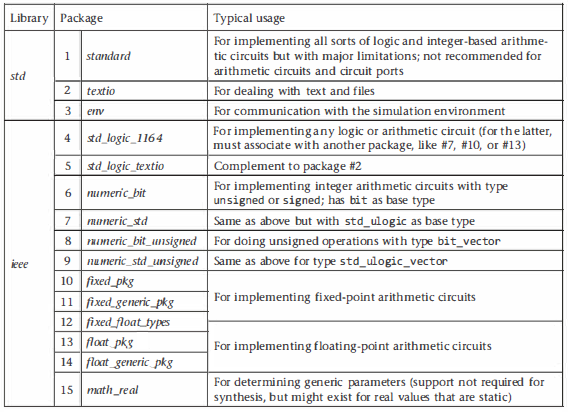
\includegraphics[width=0.7\textwidth]{Figs/fig28.png}
	\end{figure}	
	
\end{frame}


%----------------------------------------------------------------------------------------
\begin{frame}{VHDL- pacotes std e IEEE: tipos sintetizáveis}
	\justifying
	
	
	
	\begin{figure}[h]
		\centering
		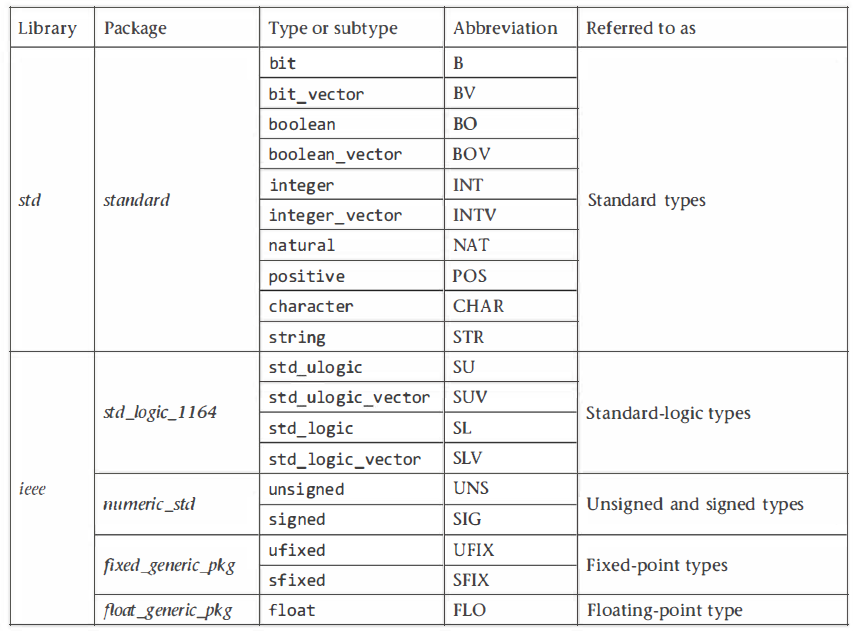
\includegraphics[width=0.65\textwidth]{Figs/fig36.png}
	\end{figure}	
	
\end{frame}


\begin{frame}{VHDL- pacotes std e IEEE}
	\justifying
	
	\begin{block}{Type STD$\_$LOGIC}
		9 logic value system (‘U’, ‘X’, ‘0’, ‘1’, ‘Z’, ‘W’, ‘L’, ‘H’, ‘-’)
		
		\begin{itemize}
			\item \textbf{1:} Logic high    
			\item \textbf{0:} Logic low
			\item \textbf{X:} Unknown
			\item \textbf{Z:} (not ‘z’) Tri-state
			\item \textbf{-:} Don’t Care
			\item \textbf{U:} Undefined
			\item \textbf{H:} Weak logic high
			\item \textbf{L:} Weak logic low
			\item \textbf{W:} Weak unknown
		\end{itemize}		
		
		
	\end{block}
	
	
	
	
	
	
\end{frame}


\begin{frame}{Conversão de tipos de dados}
	\justifying
	
	
	
	\begin{figure}[h]
		\centering
		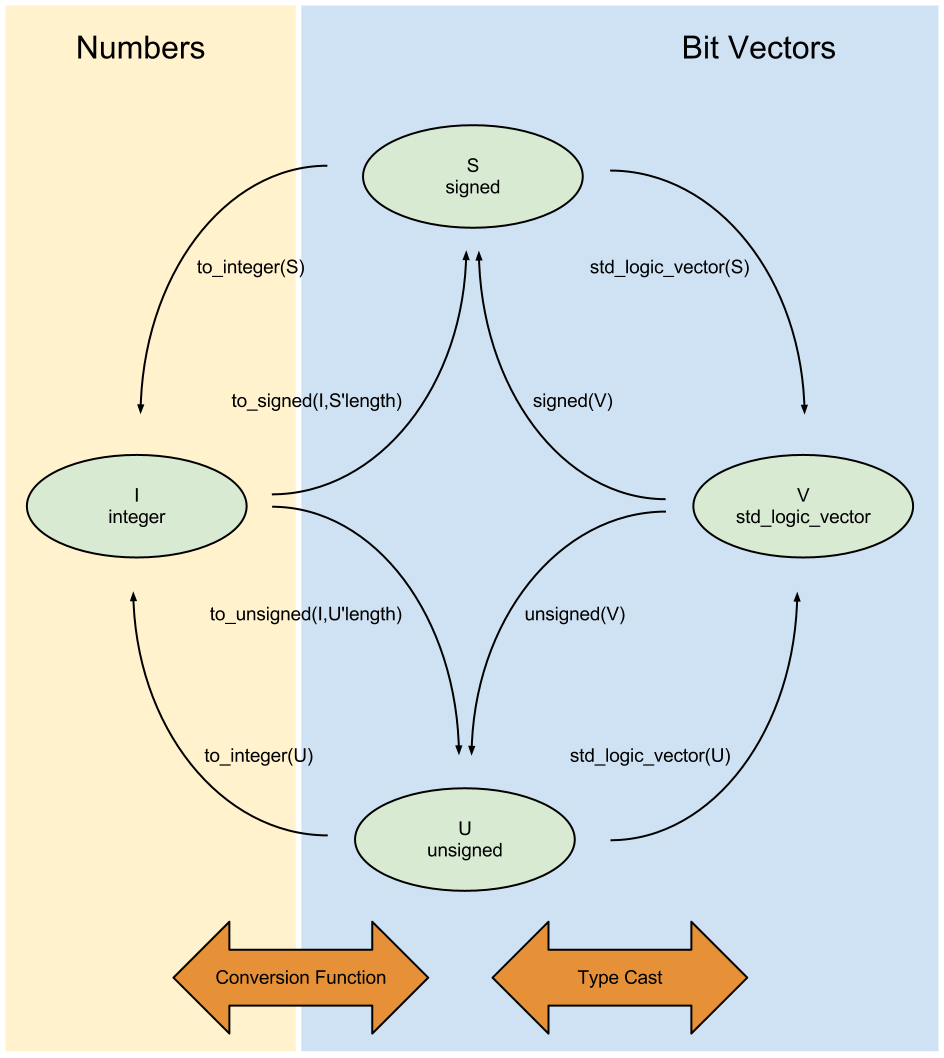
\includegraphics[width=0.45\textwidth]{Figs/vhdl-type-conversions.png}
	\end{figure}	
	
\end{frame}


% --- FRAME 5 ---
%\begin{frame}{Declaração de Bibliotecas e Pacotes}
%	\justifying
%	Para tornar um pacote visível ao design, são necessárias duas declarações: a biblioteca onde o pacote se encontra e uma cláusula \texttt{USE} apontando para o pacote específico.
%	
%	\begin{itemize}
%		\item \textbf{std} e \textbf{work}: São visíveis por padrão e não precisam ser declaradas explicitamente.
%		\item \textbf{ieee}: Deve ser declarada sempre que tipos como \texttt{STD\_LOGIC} forem utilizados.
%	\end{itemize}
%	
%	\begin{figure}[h]
%		\centering
%		%\includegraphics[width=0.6\textwidth]{Figs/fig_declaracao.png} 
%		\caption{Sintaxe de declaração de biblioteca e pacotes.}
%	\end{figure}
%\end{frame}














%
%% --- FRAME 6 ---
%\begin{frame}{A Unidade \texttt{ENTITY}}
%	\justifying
%	A parte principal de uma \texttt{ENTITY} é o \texttt{PORT}, que lista todas as especificações de pinos (entradas e saídas) do circuito.
%	
%	Cada porta deve possuir um nome, um \textbf{modo} (direção) e um \textbf{tipo} de dado. A sintaxe simplificada define a interface física que o mundo exterior "enxerga" do componente.
%	
%	\begin{figure}[h]
%		\centering
%		%\includegraphics[width=0.6\textwidth]{Figs/fig_sintaxe_entity.png} 
%		\caption{Sintaxe simplificada da declaração de ENTITY.}
%	\end{figure}
%\end{frame}

% --- FRAME 7 ---
%\begin{frame}{Exemplo de \texttt{ENTITY}}
%	\justifying
%	Considere uma porta NAND de duas entradas. A entidade define que o circuito possui três portas: duas de entrada (\texttt{a} e \texttt{b}) e uma de saída (\texttt{x}), todas do tipo \texttt{BIT}.
%	
%	\begin{figure}[h]
%		\centering
%		%\includegraphics[width=0.6\textwidth]{Figs/fig_nand_modes.png} 
%		\caption{(a) Modos de porta em VHDL; (b) Representação da porta NAND.}
%	\end{figure}
%	
%	\begin{figure}[h]
%		\centering
%		%\includegraphics[width=0.6\textwidth]{Figs/fig_exemplo_entity_code.png} 
%		\caption{Exemplo de código para a entidade \texttt{nand\_gate}.}
%	\end{figure}
%\end{frame}



%\begin{frame}{Corpo da arquitetura}
%	\justifying
%	
%	
%	\begin{block}{}
%		\justifying
%		A ``ARCHITECTURE" em VHDL é usada para definir o comportamento ou a estrutura interna de um componente digital descrito na linguagem. 
%		
%		\begin{itemize}
%			\item Descreve a funcionalidade.
%			\item Declarações são executadas concorrentemente (processos).
%			\item Podem ser colocadas várias arquiteturas.
%			\item \textbf{Behavioral:} mostra como funciona.
%			\item \textbf{RTL:} A descrição dos designs é feita em termos de registradores.
%			\item \textbf{Hybrid:} mistura de ambos estilos.
%		\end{itemize}	
%		
%	\end{block}	
%	
%	
%	
%\end{frame}










%\begin{frame}{VHDL- Estrutura Básica de Modelagem}
%	\justifying
%	
%	
%	\begin{figure}[h]
%		\centering
%		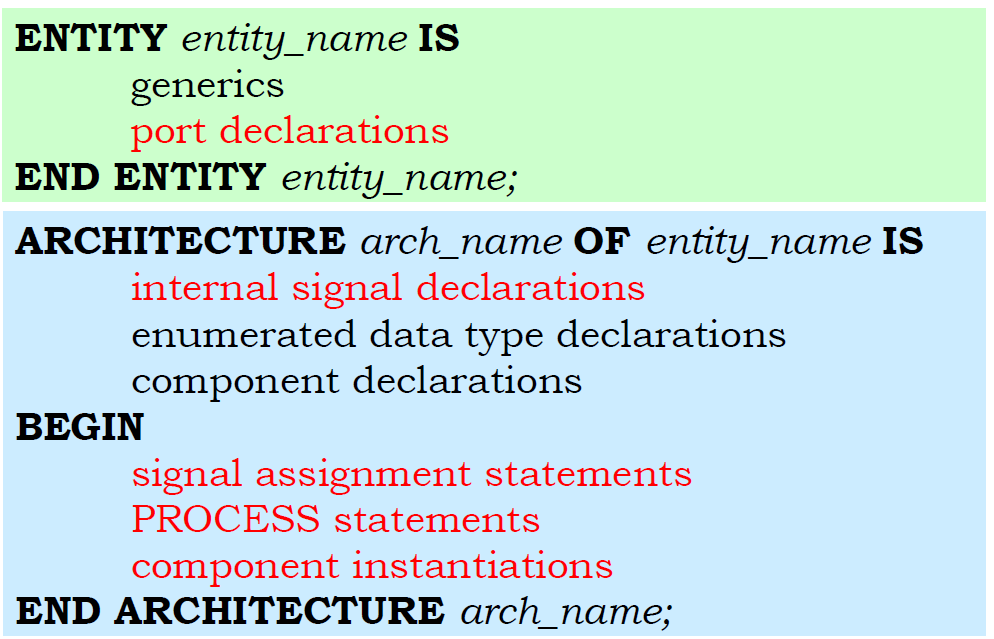
\includegraphics[width=0.77\textwidth]{Figs/fig16.png}
%	\end{figure}
%	
%	
%	
%\end{frame}






%\begin{frame}{Definição de novos tipos}
%	\justifying
%	
%	\begin{block}{}
%		\justifying
%		A linguagem VHDL permite a criação de novos tipos enumerados, físicos e compostos.
%	\end{block}		
%	
%	\begin{figure}[h]
%		\centering
%		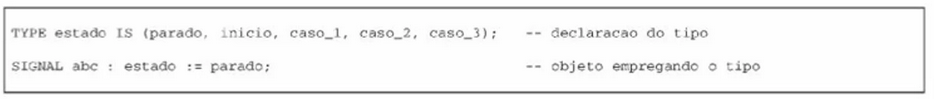
\includegraphics[width=0.97\textwidth]{Figs/fig23.png}
%	\end{figure}
%	
%	%	\begin{block}{Subtype}
%		%	\justifying
%		%	Sintetizável se o tipo base é sintetizável.
%		%	\end{block}		
%	%	
%	%	\begin{figure}[h]
%		%		\centering
%		%		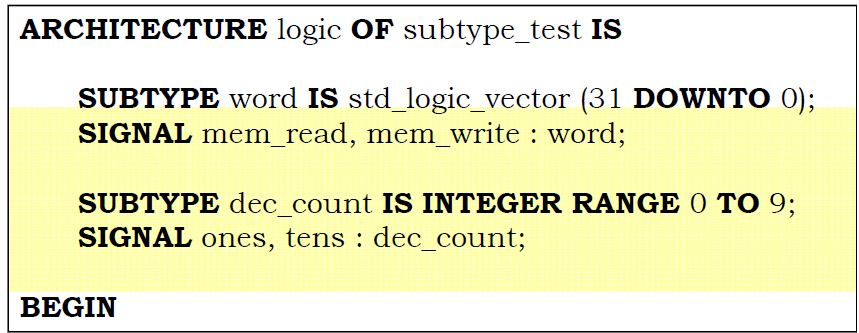
\includegraphics[width=0.57\textwidth]{Figs/fig73.png}
%		%	\end{figure}
%	
%\end{frame}


%\begin{frame}{Definição de novos tipos}
%	\justifying
%	%	
%	%	\begin{block}{}
%		%		\justifying
%		%		A linguagem VHDL permite a criação de novos tipos enumerados, físicos e compostos.
%		%	\end{block}		
%	%	
%	%	\begin{figure}[h]
%		%		\centering
%		%		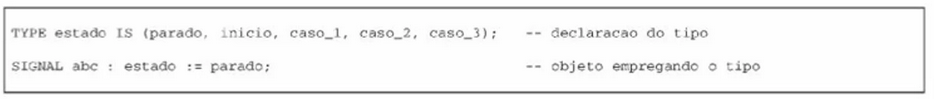
\includegraphics[width=0.97\textwidth]{Figs/fig23.png}
%		%	\end{figure}
%	
%	\begin{block}{Subtype}
%		\justifying
%		Sintetizável se o tipo base é sintetizável.
%	\end{block}		
%	
%	\begin{figure}[h]
%		\centering
%		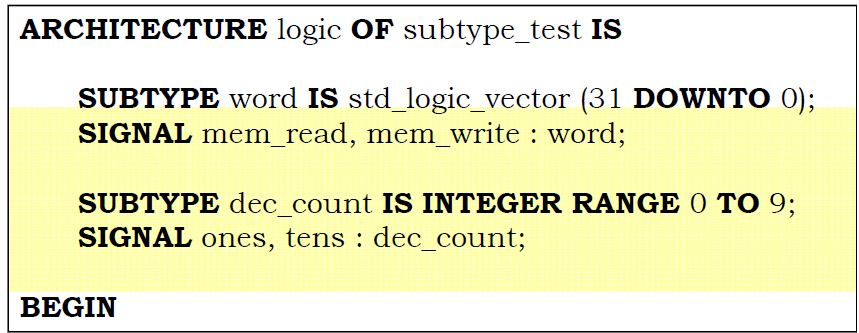
\includegraphics[width=0.57\textwidth]{Figs/fig73.png}
%	\end{figure}
%	
%\end{frame}



\begin{frame}{Operadores}
	\justifying
	
	\begin{block}{}
		\justifying
		Os operadores definidos são divididos em classes que estabelecem a precedência na execução das operações.
	\end{block}		
	
	\begin{figure}[h]
		\centering
		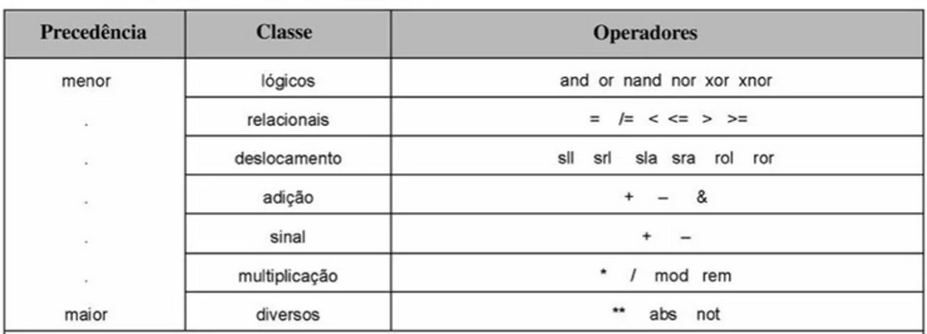
\includegraphics[width=0.9\textwidth]{Figs/fig24.png}
	\end{figure}
	
	
\end{frame}




\begin{frame}{Operadores}
	\justifying
	
	
	\begin{figure}[h]
		\centering
		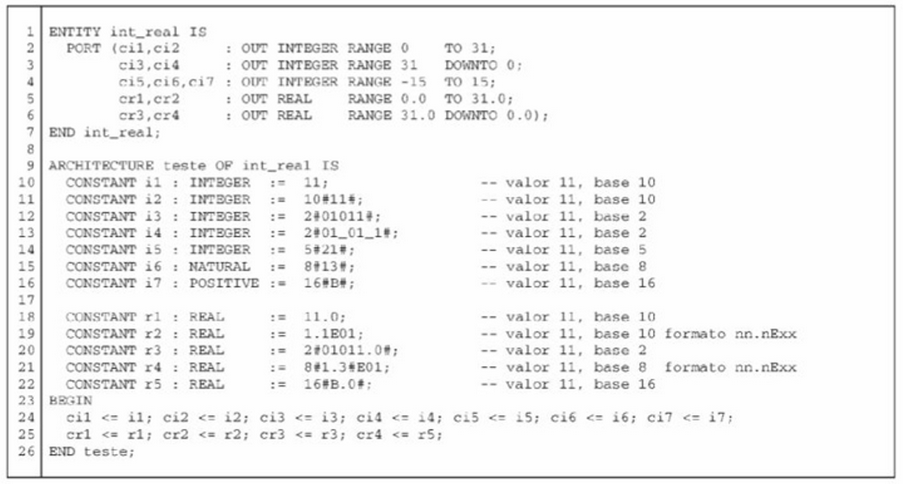
\includegraphics[width=0.9\textwidth]{Figs/fig25.png}
	\end{figure}
	
	
\end{frame}

%----------------------------------------------------------------------------------------
\begin{frame}{Operadores}
	\justifying
	
	
	\begin{figure}[h]
		\centering
		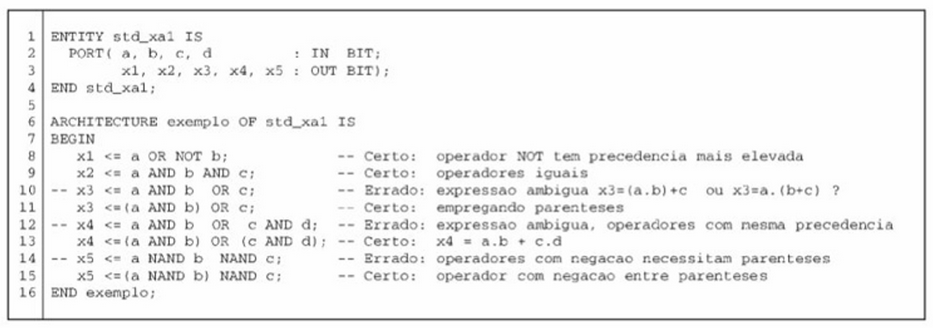
\includegraphics[width=0.9\textwidth]{Figs/fig26.png}
	\end{figure}
	
	
\end{frame}
%----------------------------------------------------------------------------------------
\begin{frame}{Operadores}
	\justifying
	
	
	\begin{figure}[h]
		\centering
		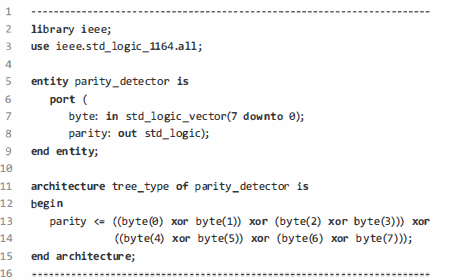
\includegraphics[width=0.77\textwidth]{Figs/fig30.png}
	\end{figure}
	
	
\end{frame}
%----------------------------------------------------------------------------------------
\begin{frame}{Operadores: sinais usadas como interligação}
	\justifying
	
	
	\begin{figure}[h]
		\centering
		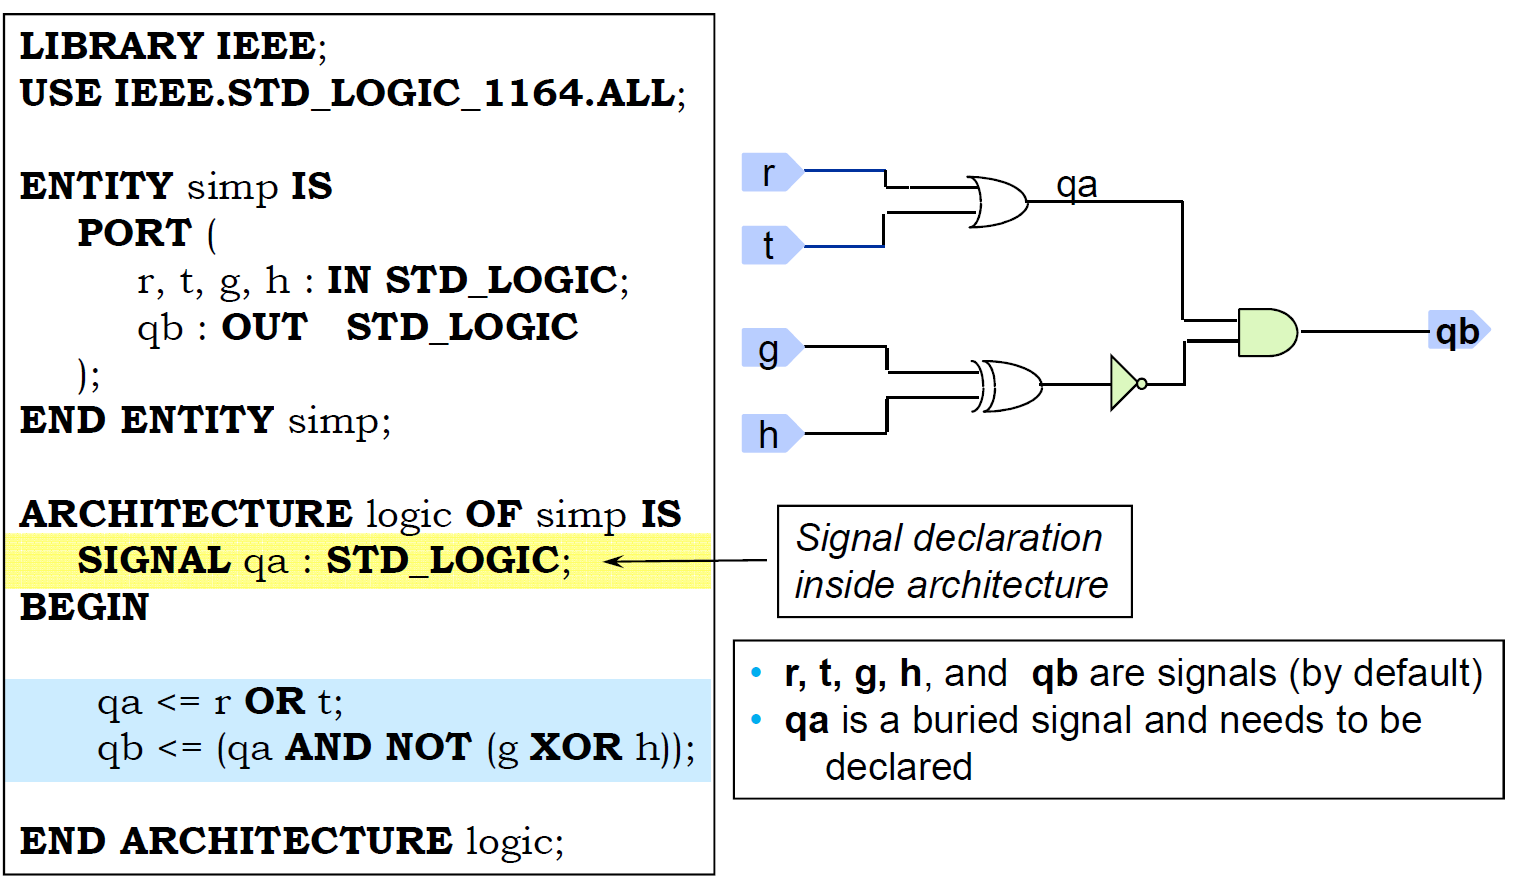
\includegraphics[width=0.77\textwidth]{Figs/fig32.png}
	\end{figure}
	
	
\end{frame}
%----------------------------------------------------------------------------------------
\begin{frame}{Operadores: função aritmética}
	\justifying
	
	
	\begin{figure}[h]
		\centering
		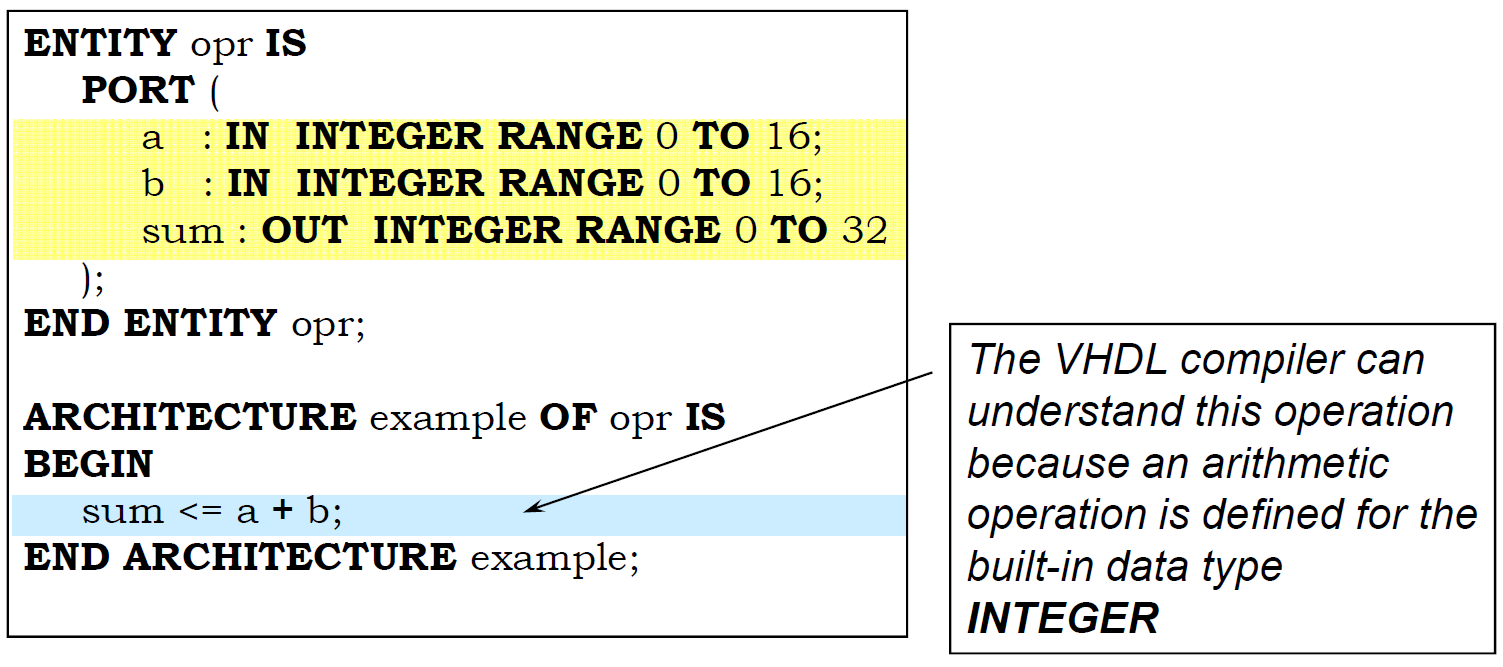
\includegraphics[width=0.77\textwidth]{Figs/fig33.png}
	\end{figure}
	
	
\end{frame}











\section{Declarações Concorrentes}
%----------------------------------------------------------------------------------------
\begin{frame}{Declarações Concorrentes}
	\justifying
	
	\begin{itemize}
		\item Declaração \textbf{when}
		\item Declaração \textbf{select}
		\item Declaração \textbf{generate}
		\item Declaração \textbf{Process}
	\end{itemize}
	
	
	\begin{block}{Declarações concorrentes}
		VHDL é inerentemente concorrente em vez de sequencial.	
		
	\end{block}
	
	%	\begin{figure}[h]
		%		\centering
		%		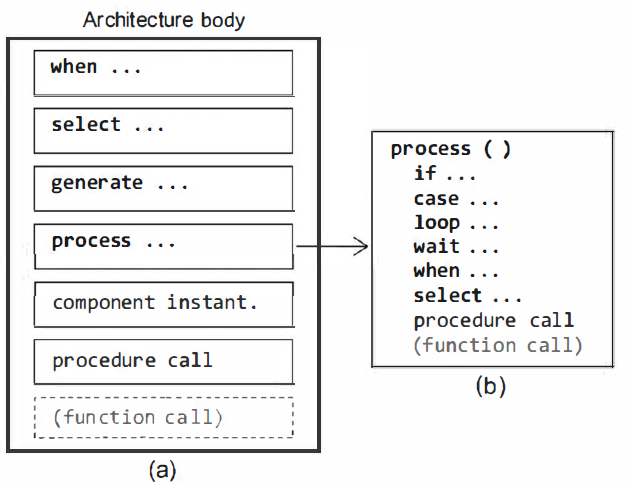
\includegraphics[width=0.57\textwidth]{Figs/fig38.png}
		%	\end{figure}
	
	
\end{frame}


\begin{frame}{Declarações Concorrentes}
	\justifying
	
	%	\begin{itemize}
		%		\item Declaração \textbf{when}
		%		\item Declaração \textbf{select}
		%		\item Declaração \textbf{generate}
		%		\item Declaração \textbf{Process}
		%	\end{itemize}
	%	
	%	
	%	\begin{block}{Declarações concorrentes}
		%		VHDL é inerentemente concorrente em vez de sequencial.	
		%		
		%	\end{block}
	
	\begin{figure}[h]
		\centering
		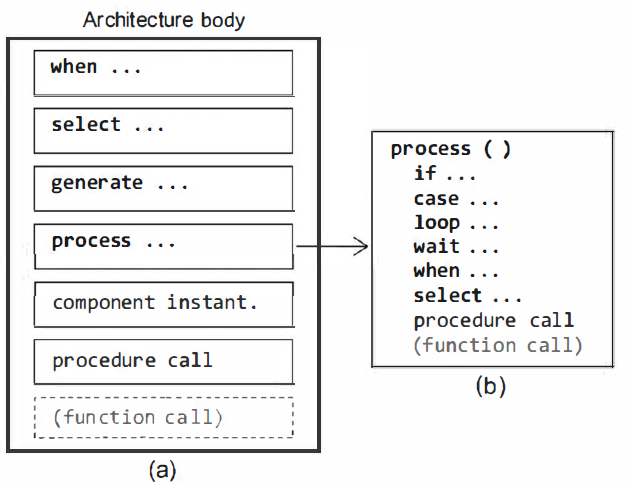
\includegraphics[width=0.57\textwidth]{Figs/fig38.png}
	\end{figure}
	
	
\end{frame}
%----------------------------------------------------------------------------------------
%\subsection{select}
%----------------------------------------------------------------------------------------
%\begin{frame}{Declaração select}
%	\justifying
%	
%	
%	
%	
%	\begin{block}{}
%		\begin{itemize}
%			\item Todas as possíveis condições devem ser consideradas.
%			\item \textbf{when others} avalia todas as outras condições possíveis que não são especificamente declaradas.
%		\end{itemize}
%		
%	\end{block}
%	
%	\begin{figure}[h]
%		\centering
%		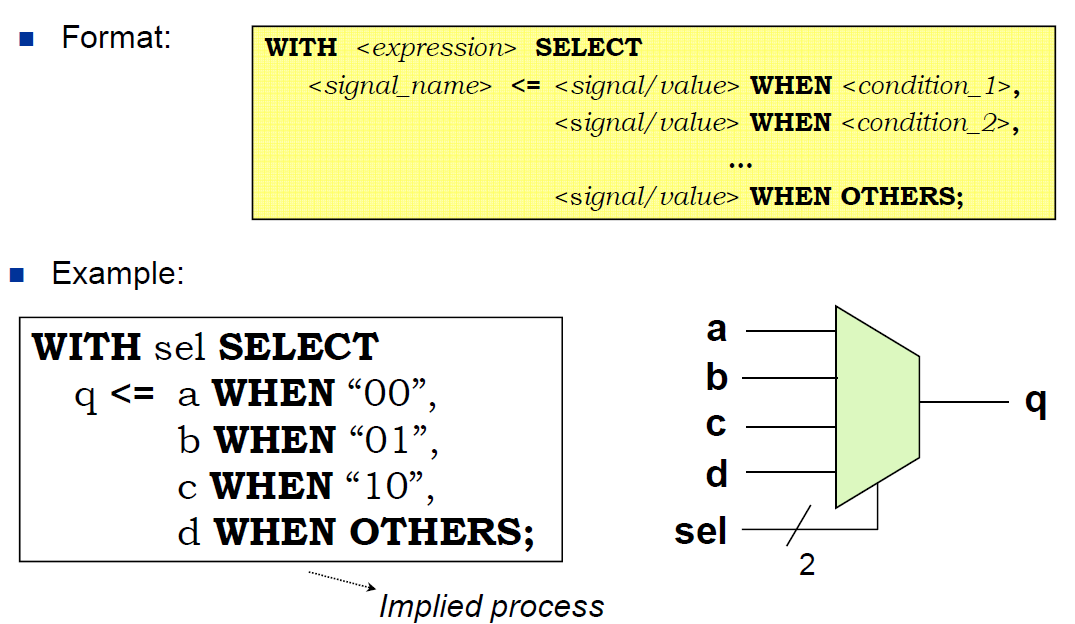
\includegraphics[width=0.57\textwidth]{Figs/fig39.png}
%	\end{figure}
%	
%	
%\end{frame}
%%----------------------------------------------------------------------------------------
%\begin{frame}{Declaração select}
%	\justifying
%	
%	
%	\begin{figure}[h]
%		\centering
%		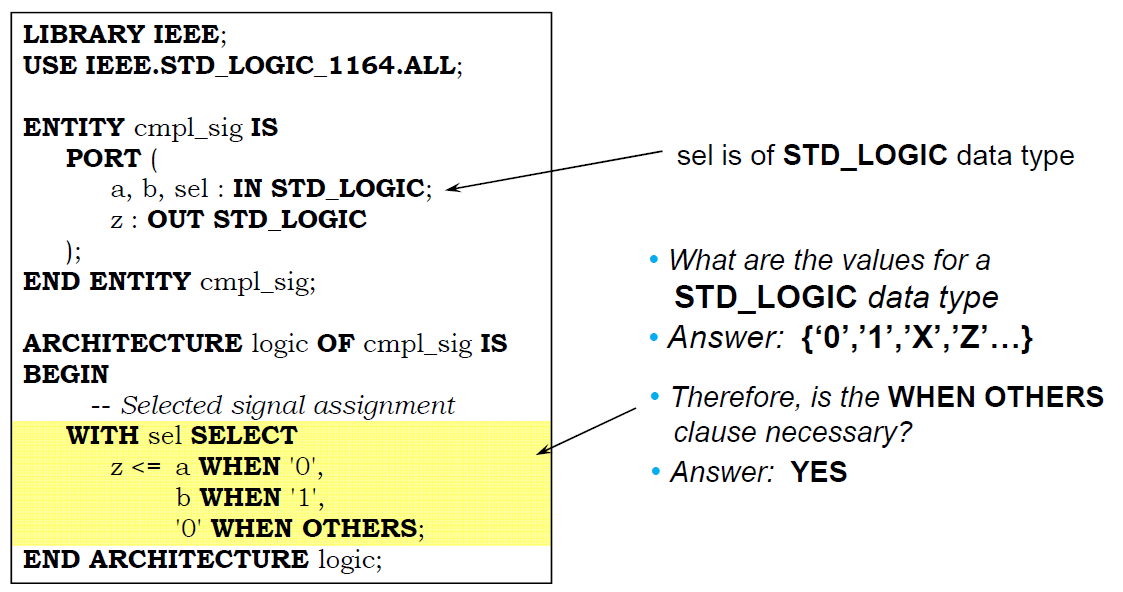
\includegraphics[width=0.77\textwidth]{Figs/fig40.png}
%	\end{figure}
%	
%	
%\end{frame}
%%----------------------------------------------------------------------------------------
%\begin{frame}{Declaração select}
%	\justifying
%	
%	
%	\begin{figure}[h]
%		\centering
%		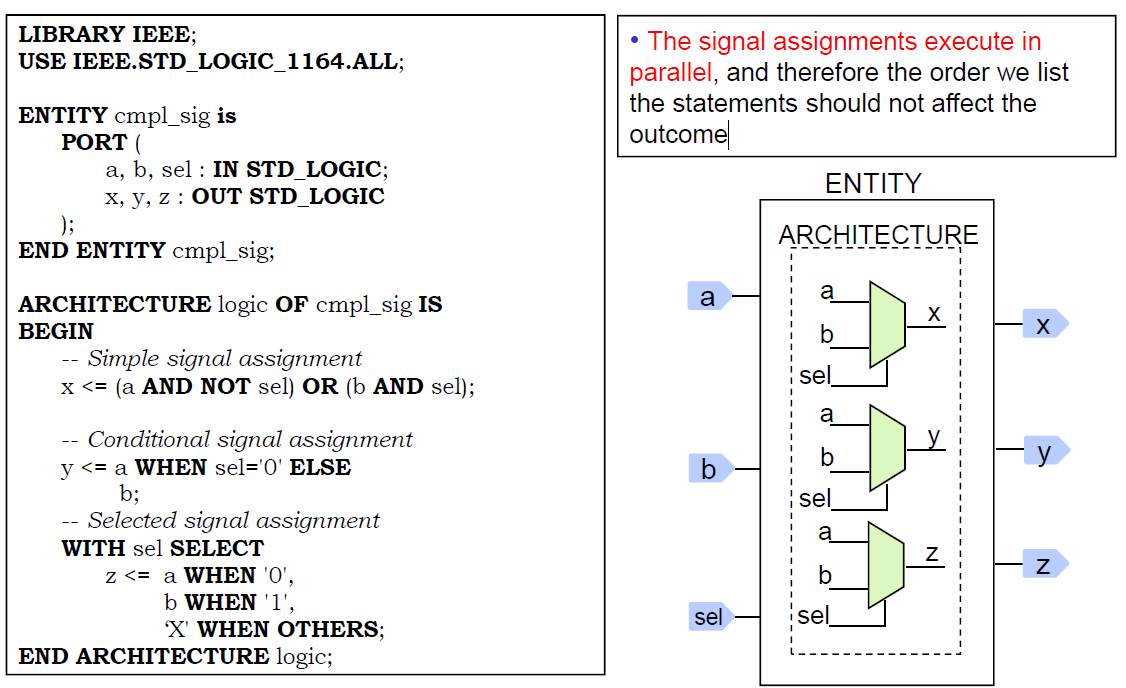
\includegraphics[width=0.77\textwidth]{Figs/fig41.png}
%	\end{figure}
%	
%	
%\end{frame}
%%----------------------------------------------------------------------------------------
%%\subsection{when}
%%----------------------------------------------------------------------------------------
%\begin{frame}{Declaração when}
%	\justifying
%	
%	
%	\begin{figure}[h]
%		\centering
%		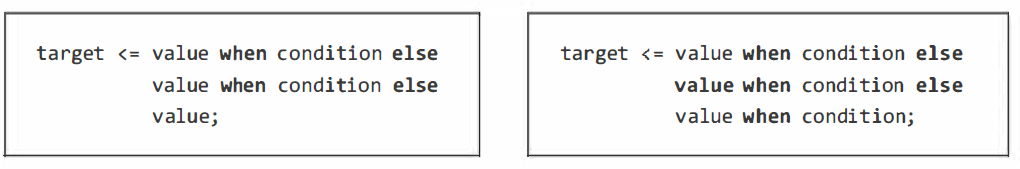
\includegraphics[width=0.97\textwidth]{Figs/fig42.png}
%	\end{figure}
%	
%	\begin{figure}[h]
%		\centering
%		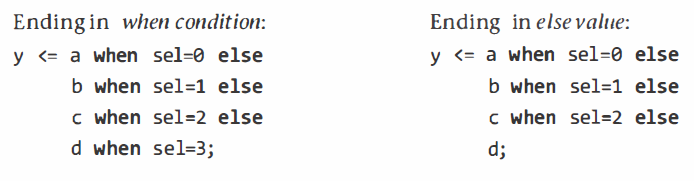
\includegraphics[width=0.57\textwidth]{Figs/fig43.png}
%	\end{figure}
%	
%\end{frame}
%%----------------------------------------------------------------------------------------
%\begin{frame}{Declaração when}
%	\justifying
%	
%	
%	\begin{figure}[h]
%		\centering
%		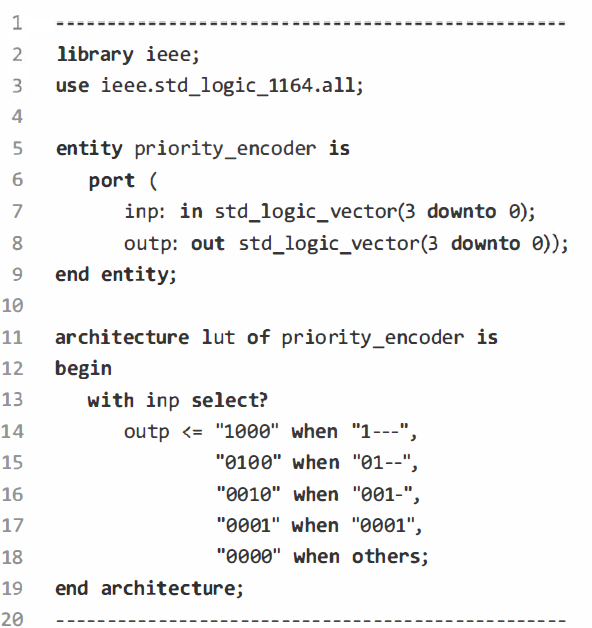
\includegraphics[width=0.47\textwidth]{Figs/fig44.png}
%	\end{figure}
%	
%	
%\end{frame}


	
	
%----------------------------------------------------------------------------------------
\begin{frame}{Instanciação de componentes}
	\justifying
	
	\begin{block}{}
		Refere-se ao processo de criar uma instância ou uma cópia de uma entidade (design ou componente) dentro de um design maior. Isso permite reutilizar funcionalidades já definidas em um novo contexto, evitando a necessidade de reescrever o código.
		
	\end{block}
	
	%	\begin{figure}[h]
		%		\centering
		%		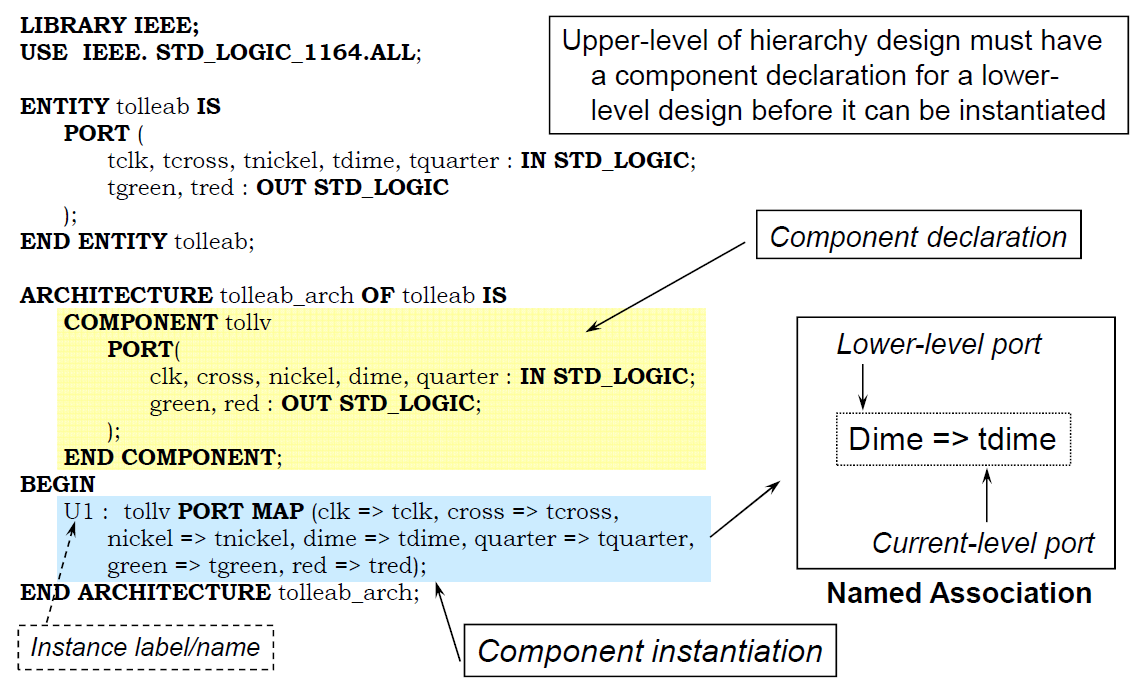
\includegraphics[width=0.67\textwidth]{Figs/fig45.png}
		%	\end{figure}
	%	
	
\end{frame}
	
	\begin{frame}{Instanciação de componentes}
		\justifying
		
		%	\begin{block}{}
			%		Refere-se ao processo de criar uma instância ou uma cópia de uma entidade (design ou componente) dentro de um design maior. Isso permite reutilizar funcionalidades já definidas em um novo contexto, evitando a necessidade de reescrever o código.
			%		
			%	\end{block}
		
		\begin{figure}[h]
			\centering
			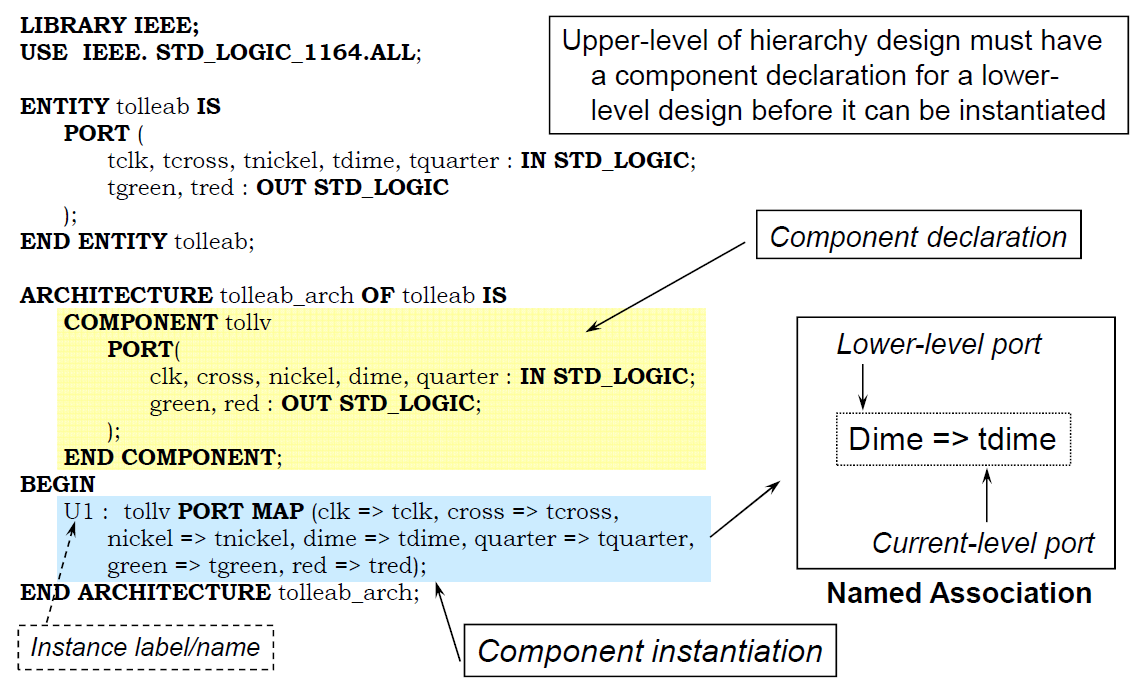
\includegraphics[width=0.77\textwidth]{Figs/fig45.png}
		\end{figure}
		
		
	\end{frame}
	
\begin{frame}{Instanciação de componentes}
	\justifying
	
	
	\begin{figure}[h]
		\centering
		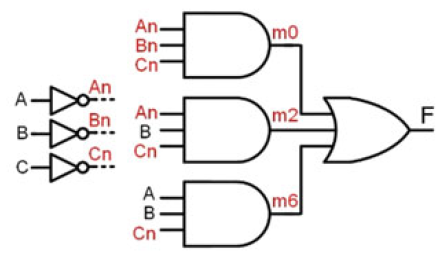
\includegraphics[width=0.5\textwidth]{Figs/fig46.png}
	\end{figure}
	
	
	%    \begin{columns}
		%	
		%	\column{0.45\textwidth}
		%	\begin{figure}[h]
			%	\centering
			%	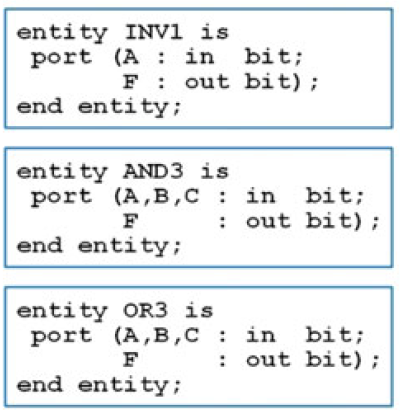
\includegraphics[width=0.47\textwidth]{Figs/fig47.png}
			%	\end{figure}
		%	
		%	\column{0.45\textwidth}
		%	\begin{figure}[h]
			%	\centering
			%	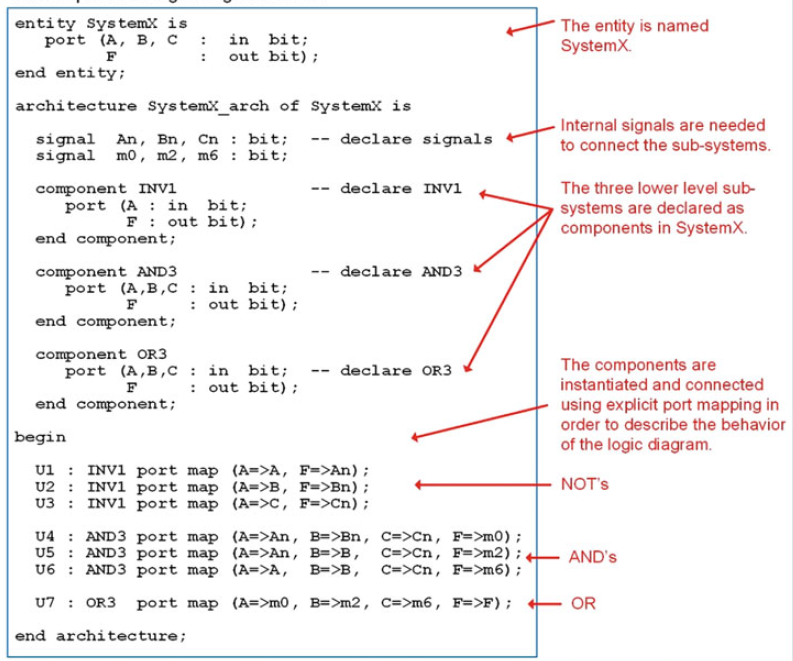
\includegraphics[width=0.97\textwidth]{Figs/fig48.png}
			%	\end{figure}
		%	\end{columns}
	
	
\end{frame}
	
\begin{frame}{Instanciação de componentes}
	\justifying
	
	
	%	\begin{figure}[h]
		%		\centering
		%		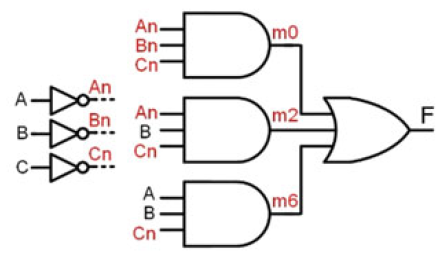
\includegraphics[width=0.37\textwidth]{Figs/fig46.png}
		%	\end{figure}
	
	
	\begin{columns}
		
		\column{0.45\textwidth}
		\begin{figure}[h]
			\centering
			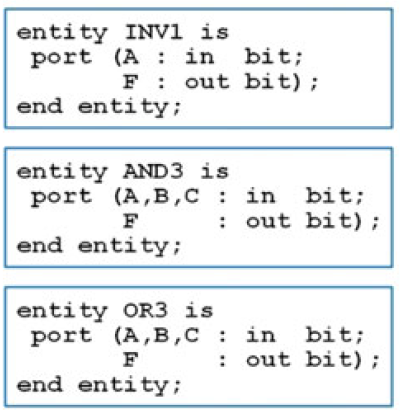
\includegraphics[width=0.57\textwidth]{Figs/fig47.png}
		\end{figure}
		
		\column{0.45\textwidth}
		\begin{figure}[h]
			\centering
			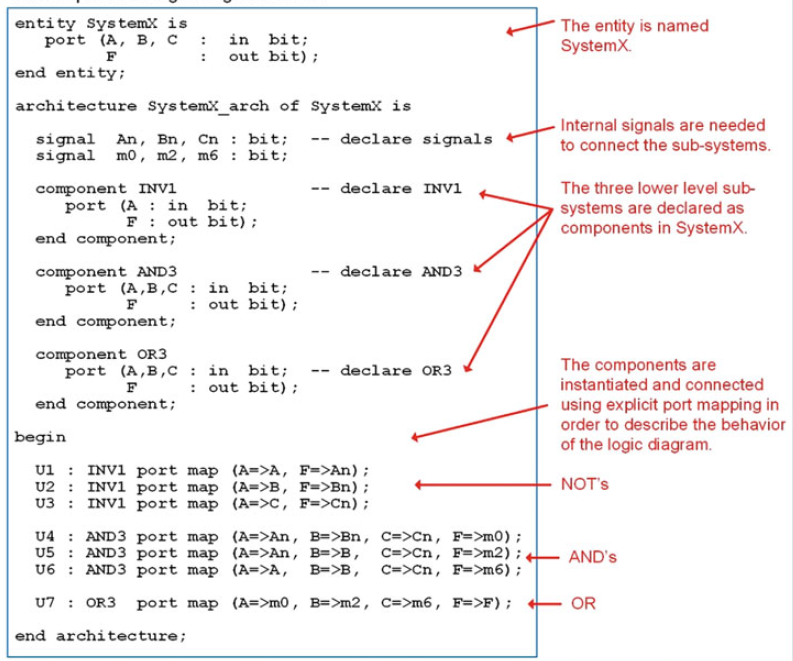
\includegraphics[width=1.1\textwidth]{Figs/fig48.png}
		\end{figure}
	\end{columns}
	
	
\end{frame}



\section{Declarações sequenciais}

\begin{frame}{Declaração de processos}
	\justifying
	
	
	\begin{block}{Process()}
		O VHDL usa um processo para modelar atribuições de sinal baseadas em um evento. Dentro de um processo em VHDL, as declarações são executadas sequencialmente. Isso significa que as instruções dentro do bloco de processo são executadas em ordem, uma após a outra, seguindo a ordem em que foram escritas no código.
	\end{block}
	
	
	\begin{block}{Sensitivity list}
		Uma lista de sensibilidade é um mecanismo para controlar quando um processo é acionado (ou iniciado). Uma lista de sensibilidade contém uma lista de sinais aos quais o processo é sensível. Se houver uma transição em qualquer um dos sinais da lista, o processo será acionado e as atribuições de sinal no processo serão feitas. 
	\end{block}	
	
	
	%	\begin{columns}
		%		
		%		\column{0.45\textwidth}
		%		\begin{figure}[h]
			%		\centering
			%		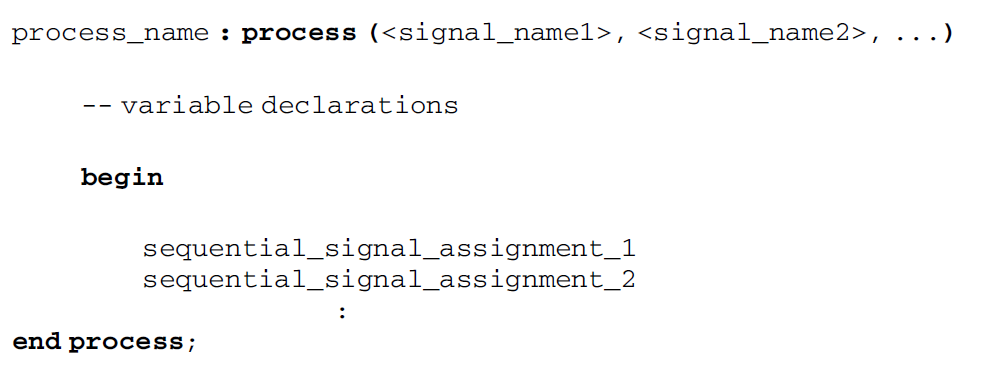
\includegraphics[width=0.97\textwidth]{Figs/fig49.png}
			%		\end{figure}
		%		
		%		\column{0.45\textwidth}
		%		\begin{figure}[h]
			%			\centering
			%			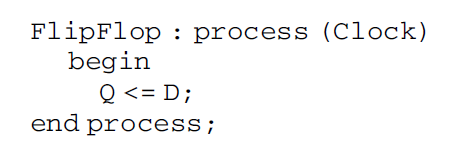
\includegraphics[width=0.57\textwidth]{Figs/fig50.png}
			%		\end{figure}
		%	\end{columns}
	%	
	
\end{frame}



\begin{frame}{Experimento 3}
	\justifying
	
Flip-flop tipo D.
	
	
\end{frame}



\begin{frame}{Declaração de processos}
	\justifying
	
	\begin{figure}[h]
		\centering
		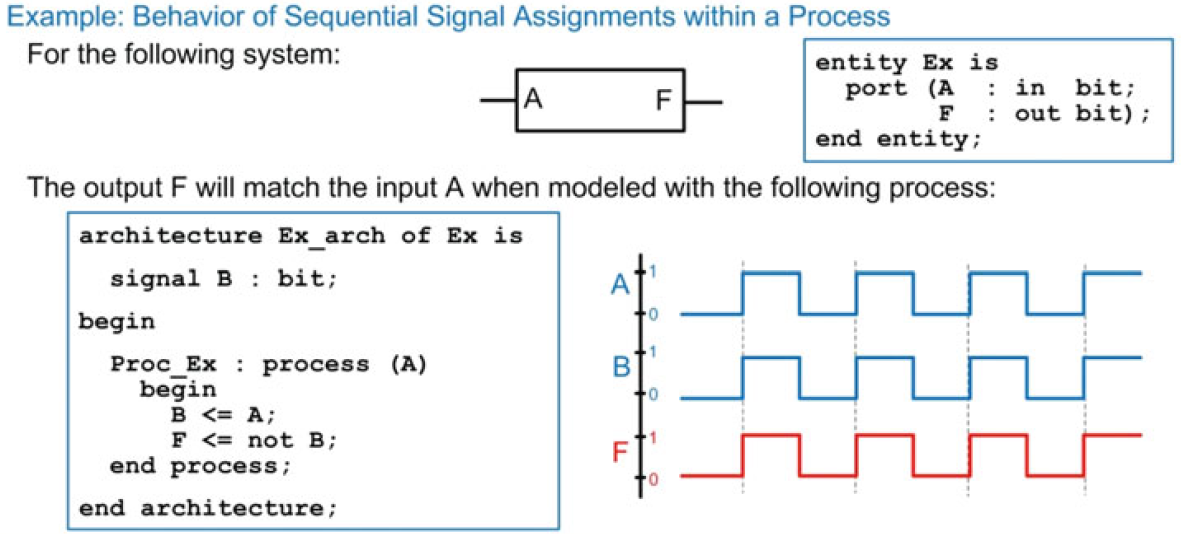
\includegraphics[width=0.67\textwidth]{Figs/fig51.png}
	\end{figure}
	
	
	
	%	\begin{figure}[h]
		%	\centering
		%	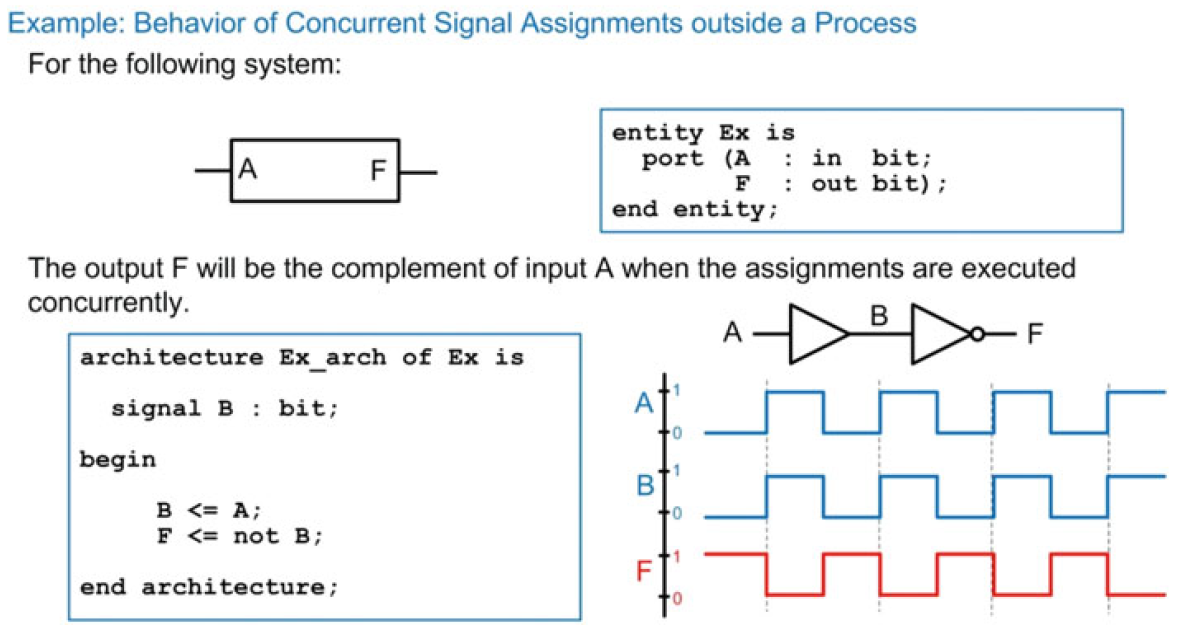
\includegraphics[width=0.67\textwidth]{Figs/fig52.png}
		%	\end{figure}	
	%	
	
	
\end{frame}


\begin{frame}{Declaração de processos}
	\justifying
	
	%	\begin{figure}[h]
		%		\centering
		%		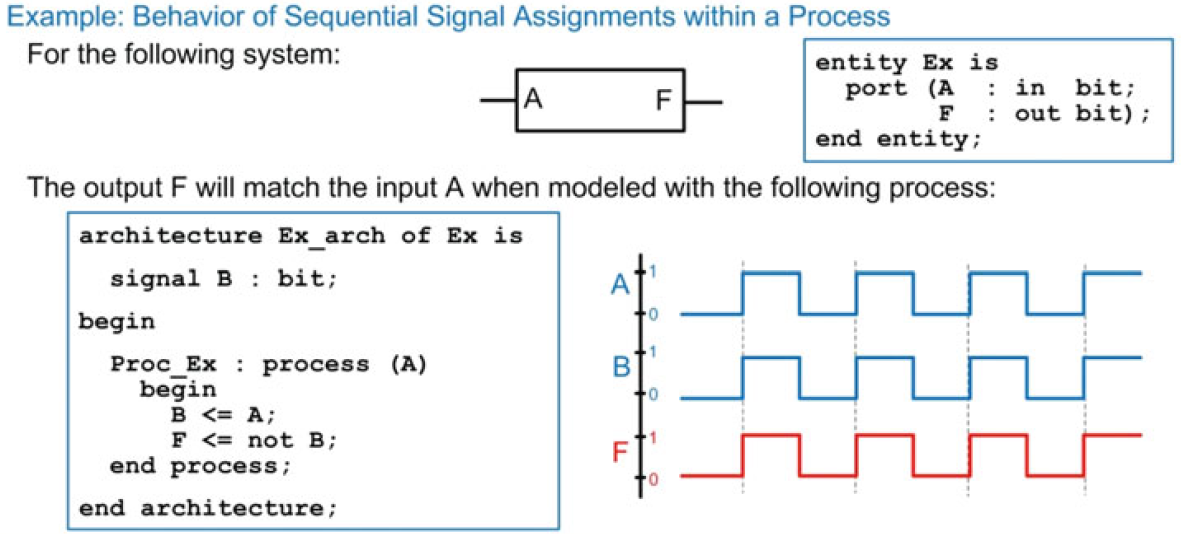
\includegraphics[width=0.67\textwidth]{Figs/fig51.png}
		%	\end{figure}
	%	
	
	
	\begin{figure}[h]
		\centering
		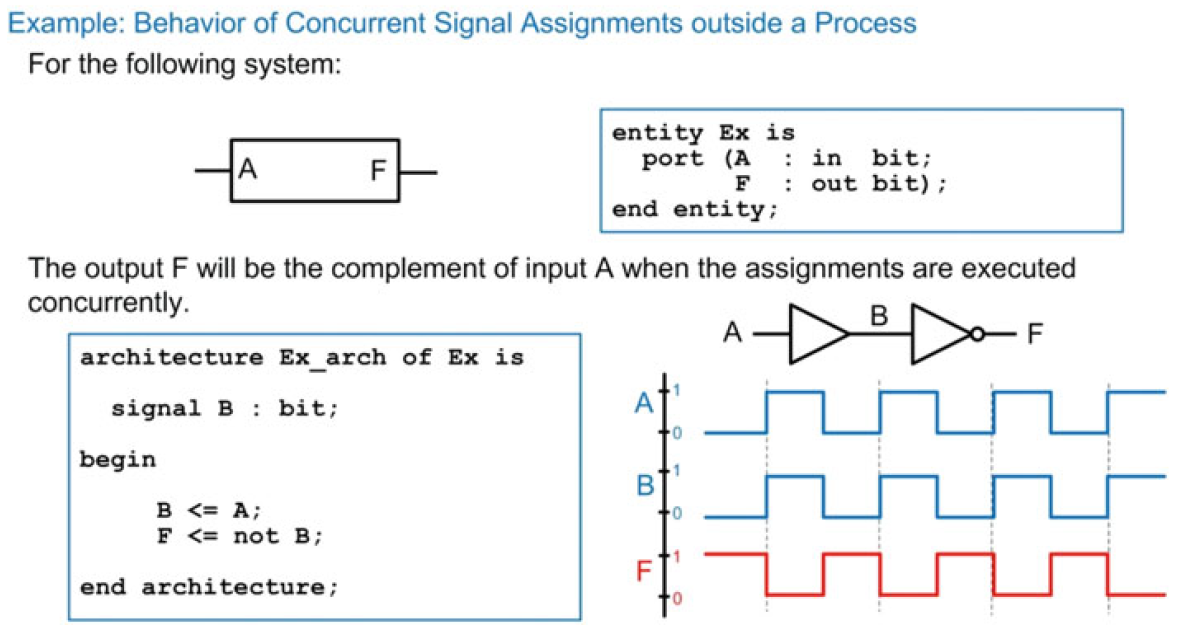
\includegraphics[width=0.67\textwidth]{Figs/fig52.png}
	\end{figure}	
	
	
	
\end{frame}


%----------------------------------------------------------------------------------------

\begin{frame}{Declaração de processos}
	\justifying
	
	\begin{figure}[h]
		\centering
		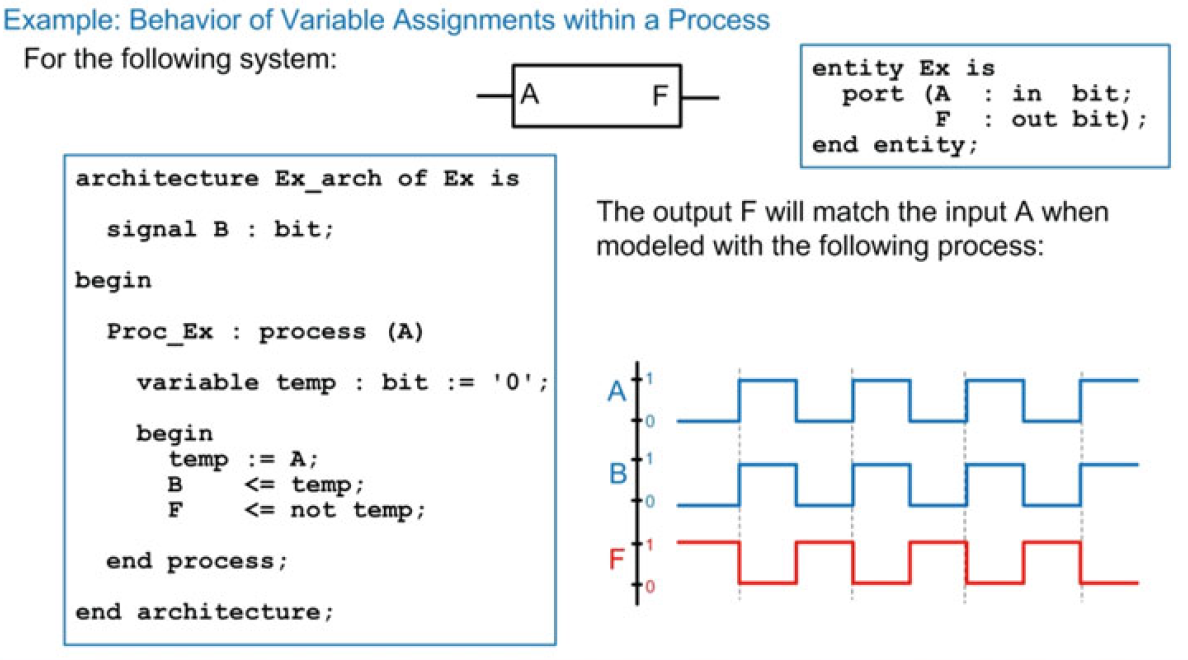
\includegraphics[width=0.67\textwidth]{Figs/fig53.png}
	\end{figure}
	
	
	
	
\end{frame}
%%----------------------------------------------------------------------------------------
\begin{frame}{Declaração de processos}
	\justifying
	
	
	\begin{block}{Processos concorrentes}
		\begin{itemize}
			\item Uma arquitetura pode ter múltiplos processos concorrentes.
			\item Cada processo é executado em paralelo com outros processos. 
			\item Sim, a ordem das declarações dentro de um processo em VHDL importa significativamente. A ordem das declarações determina a sequência de operações executadas pelo processo e pode afetar o comportamento do circuito descrito pelo código VHDL.
		\end{itemize}
		
	\end{block}		
	
	%	
	%	\begin{figure}[h]
		%		\centering
		%		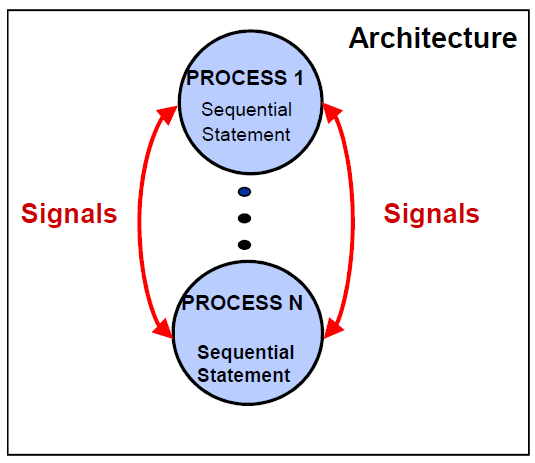
\includegraphics[width=0.47\textwidth]{Figs/fig54.png}
		%	\end{figure}
	%	
\end{frame}

\begin{frame}{Declaração de processos}
	\justifying
	
	
	%	\begin{block}{Processos concorrentes}
		%		\begin{itemize}
			%			\item Uma arquitetura pode ter múltiplos processos concorrentes.
			%			\item Cada processo é executado em paralelo com outros processos. 
			%			\item Sim, a ordem das declarações dentro de um processo em VHDL importa significativamente. A ordem das declarações determina a sequência de operações executadas pelo processo e pode afetar o comportamento do circuito descrito pelo código VHDL.
			%		\end{itemize}
		%		
		%	\end{block}		
	
	
	\begin{figure}[h]
		\centering
		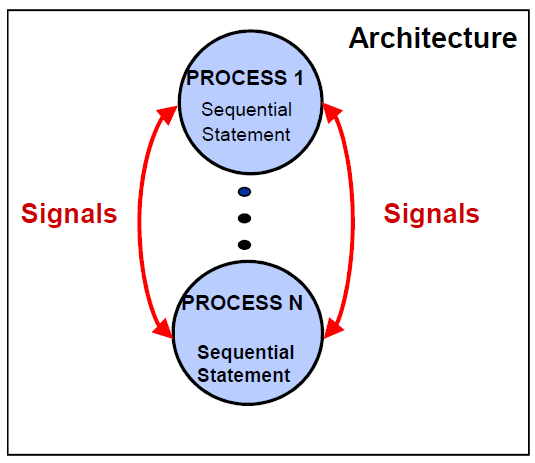
\includegraphics[width=0.47\textwidth]{Figs/fig54.png}
	\end{figure}
	
\end{frame}
	
	
\begin{frame}{Declaração de processos}
	\justifying
	
	
	\begin{figure}[h]
		\centering
		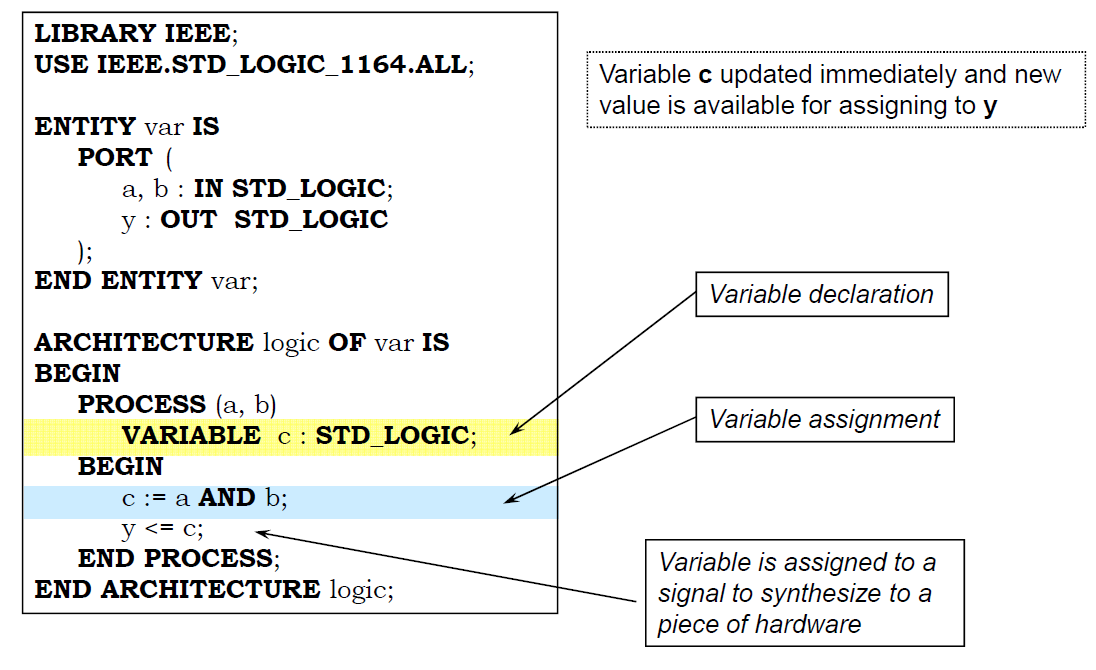
\includegraphics[width=0.77\textwidth]{Figs/fig57.png}
	\end{figure}
	
\end{frame}	
	
	
\begin{frame}{Signals vs Variables}
	\justifying
	
	
	\begin{figure}[h]
		\centering
		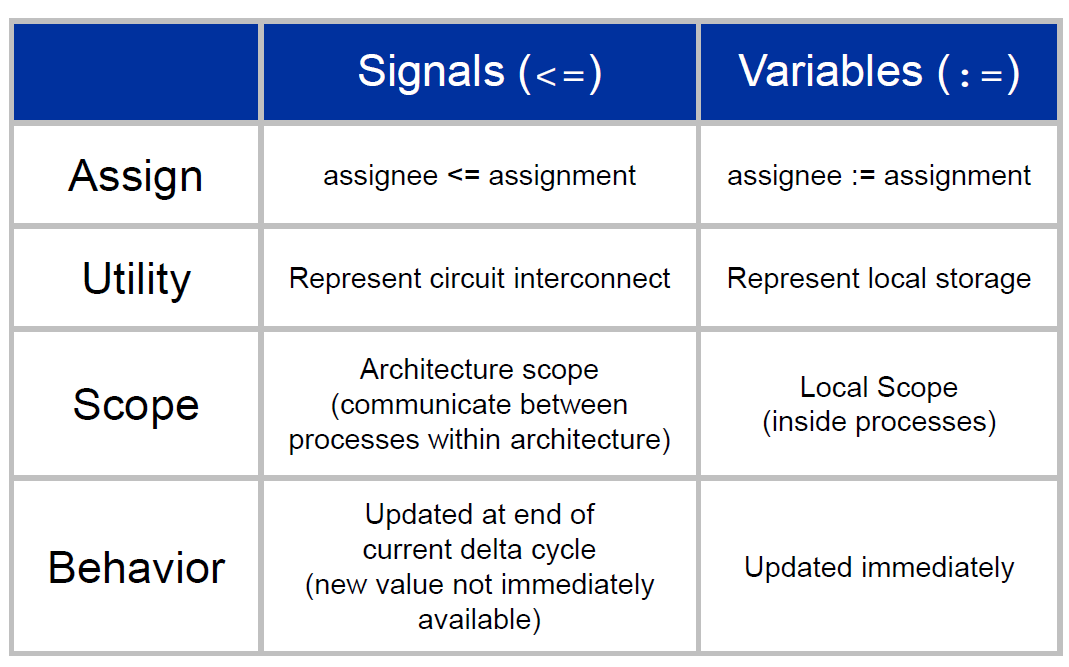
\includegraphics[width=0.77\textwidth]{Figs/fig59.png}
	\end{figure}
	
\end{frame}	
	

%%----------------------------------------------------------------------------------------
\begin{frame}{Declarações sequenciais}
	\justifying
	
	Declarações sequenciais devem estar dentro de processos.
	
	\begin{block}{}
		\begin{itemize}
			\item IF-THEN
			\item CASE 
			\item Looping statements
			\item WAIT
		\end{itemize}
		
	\end{block}		
	
	
	
\end{frame}
%%----------------------------------------------------------------------------------------
%\subsection{Declarações IF-THEN}
%%----------------------------------------------------------------------------------------
\begin{frame}{Declarações IF-THEN}
	\justifying
	
	\begin{figure}[h]
		\centering
		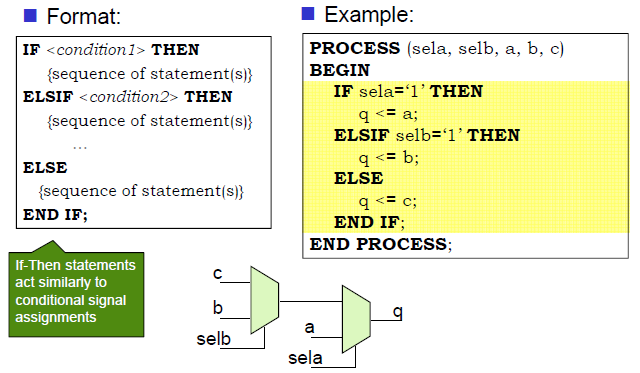
\includegraphics[width=0.87\textwidth]{Figs/fig60.png}
	\end{figure}
	
	
	
\end{frame}	
	
\begin{frame}{Declarações IF-THEN}
	\justifying
	
	\begin{figure}[h]
		\centering
		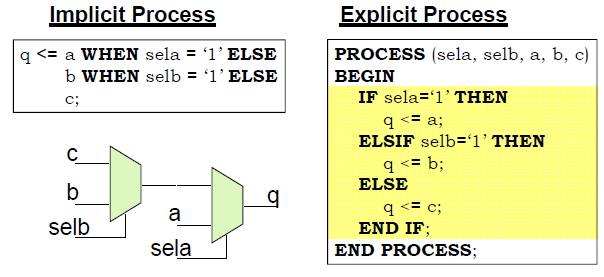
\includegraphics[width=0.87\textwidth]{Figs/fig61.png}
	\end{figure}
	
	
	
\end{frame}	

\begin{frame}{Declaração CASE}
	\justifying
	
	
	\begin{block}{}
		\begin{itemize}
			\item Todas as condições são avaliadas ao mesmo tempo.
			\item Todas as possíveis condições devem ser consideradas. 
			\item \textbf{``WHEN OTHERS"} avalia todas as outras condições possíveis que não são especificamente declaradas.
		\end{itemize}
		
	\end{block}	
	
	%	\begin{figure}[h]
		%		\centering
		%		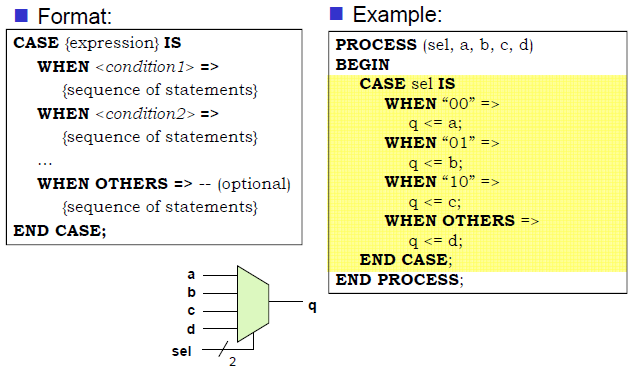
\includegraphics[width=0.87\textwidth]{Figs/fig62.png}
		%	\end{figure}
	
	
	
\end{frame}


\begin{frame}{Declaração CASE}
	\justifying
	
	
	%	\begin{block}{}
		%		\begin{itemize}
			%			\item Todas as condições são avaliadas ao mesmo tempo.
			%			\item Todas as possíveis condições devem ser consideradas. 
			%			\item \textbf{``WHEN OTHERS"} avalia todas as outras condições possíveis que não são especificamente declaradas.
			%		\end{itemize}
		%		
		%	\end{block}	
	
	\begin{figure}[h]
		\centering
		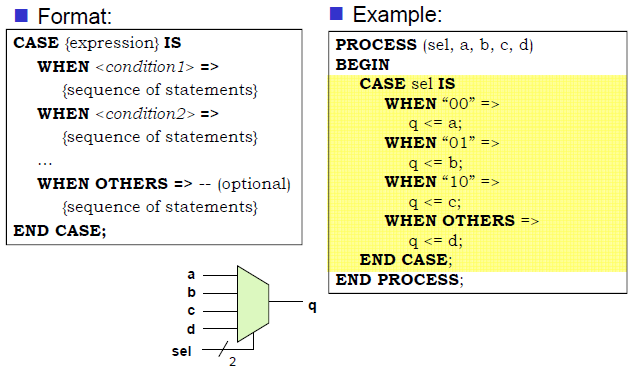
\includegraphics[width=0.87\textwidth]{Figs/fig62.png}
	\end{figure}
	
	
	
\end{frame}




%\section{VHDL and Logic Synthesis}
%%----------------------------------------------------------------------------------------
\begin{frame}{VHDL and Logic Synthesis}
	\justifying
	
	
	\begin{figure}[h]
		\centering
		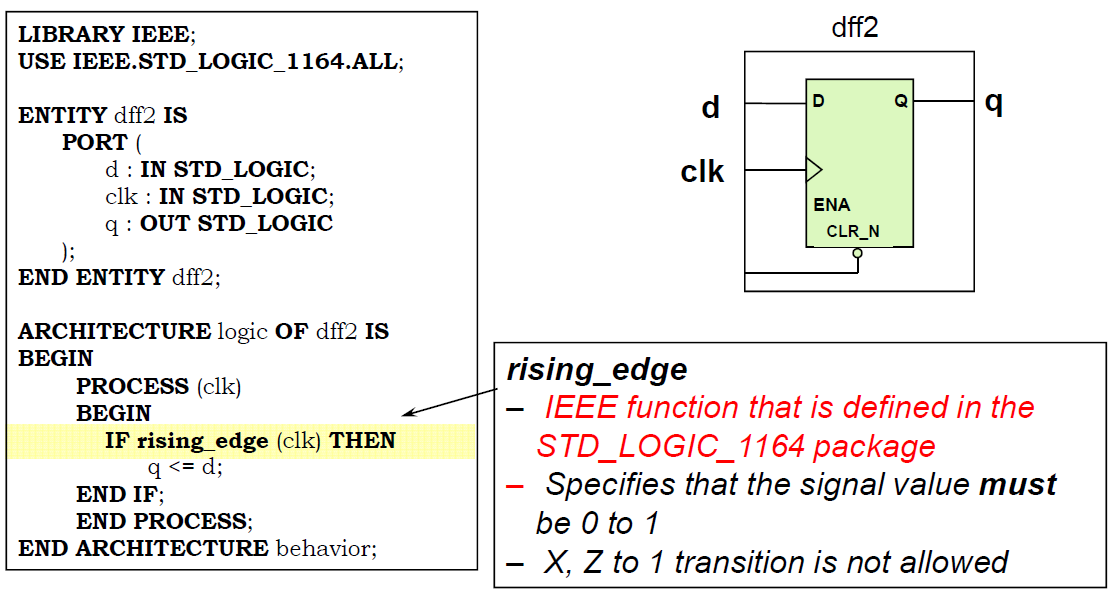
\includegraphics[width=0.87\textwidth]{Figs/fig74.png}
	\end{figure}
	
\end{frame}
%%----------------------------------------------------------------------------------------
\begin{frame}{VHDL and Logic Synthesis}
	\justifying
	
	
	\begin{figure}[h]
		\centering
		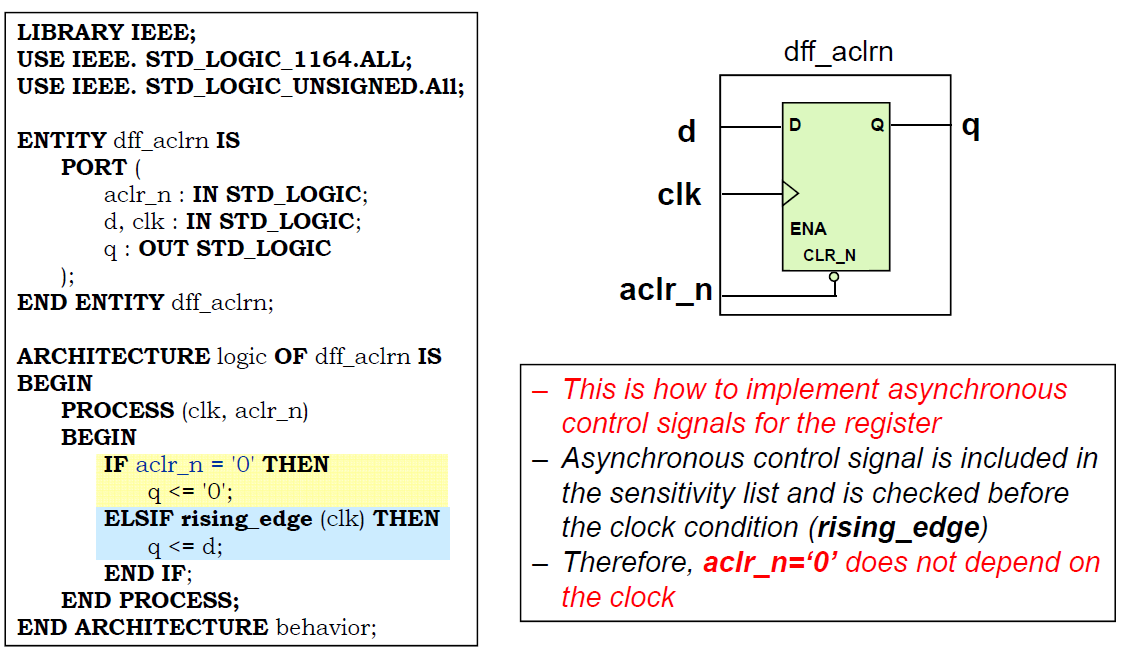
\includegraphics[width=0.87\textwidth]{Figs/fig75.png}
	\end{figure}
	
\end{frame}
%%----------------------------------------------------------------------------------------
\begin{frame}{VHDL and Logic Synthesis}
	\justifying
	
	
	\begin{figure}[h]
		\centering
		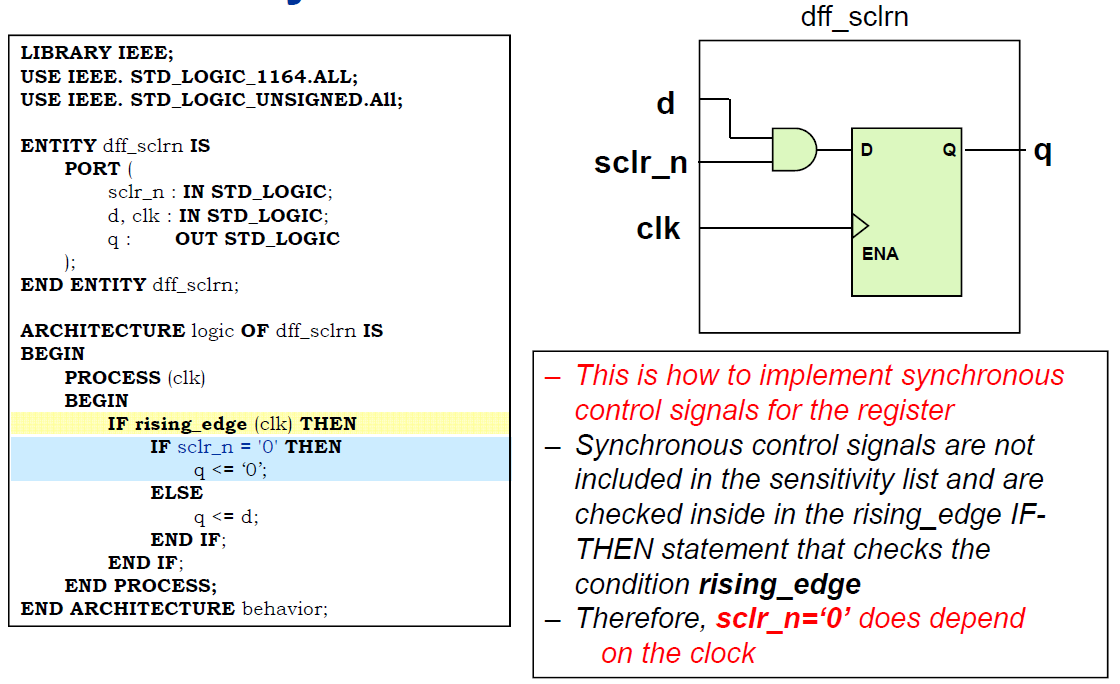
\includegraphics[width=0.77\textwidth]{Figs/fig76.png}
	\end{figure}
	
\end{frame}

%%----------------------------------------------------------------------------------------
\begin{frame}{VHDL and Logic Synthesis}
	\justifying
	
	
	\begin{figure}[h]
		\centering
		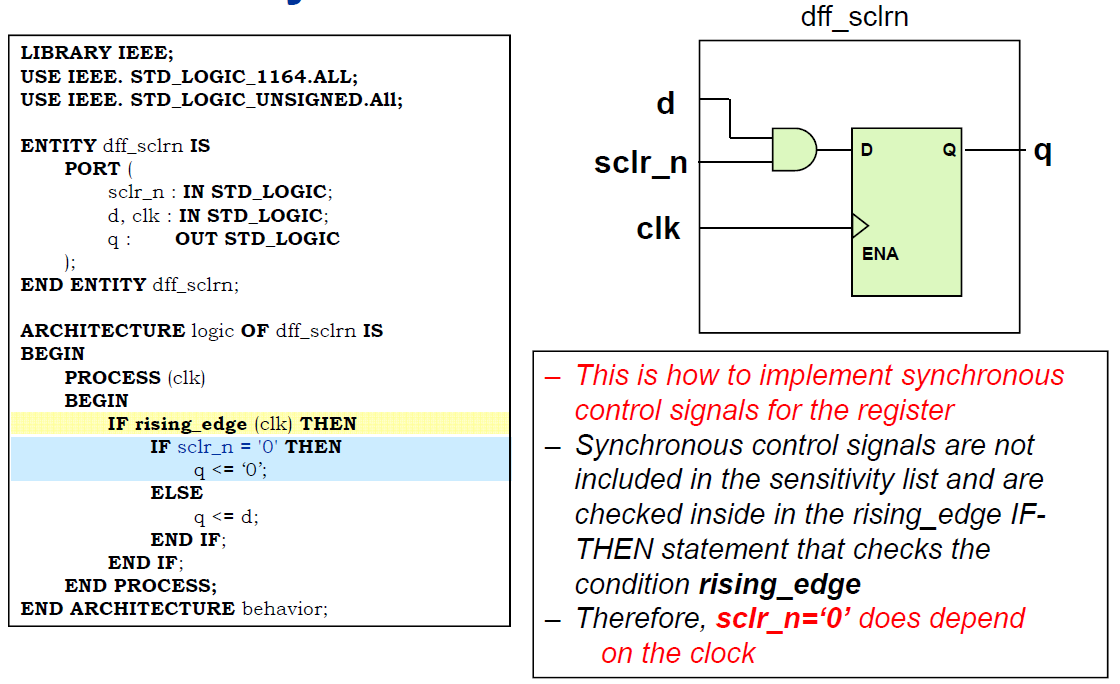
\includegraphics[width=0.77\textwidth]{Figs/fig76.png}
	\end{figure}
	
\end{frame}
%%----------------------------------------------------------------------------------------
\begin{frame}{VHDL and Logic Synthesis}
	\justifying
	
	Quantos registradores?
	
	\begin{figure}[h]
		\centering
		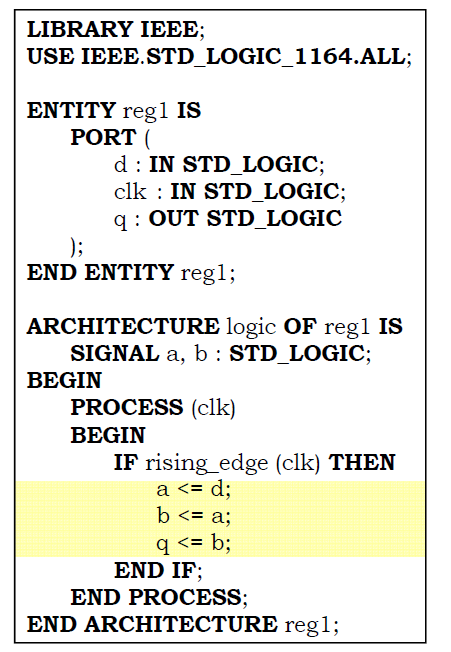
\includegraphics[width=0.32\textwidth]{Figs/fig77.png}
	\end{figure}
	
\end{frame}
%%----------------------------------------------------------------------------------------
\begin{frame}{VHDL and Logic Synthesis}
	\justifying
	
	
	\begin{figure}[h]
		\centering
		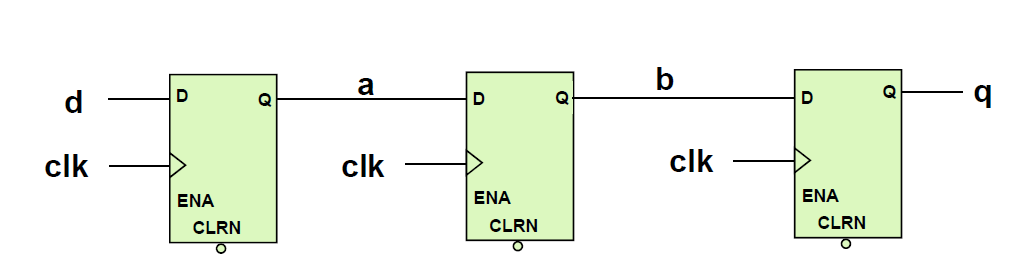
\includegraphics[width=0.87\textwidth]{Figs/fig78.png}
	\end{figure}
	
\end{frame}



\begin{frame}{Experimento 4}
	\justifying
	
	Contador de 32-bits.
	
\end{frame}

\end{document}
